\chapter{R Package singleCellFeatures}
\label{ch:singlecellfeatures}

The format in which CellProfiler feature data is stored is only of limited suitability for exploratory data analysis. CellProfiler was originally implemented in the proprietary MATLAB language but has recently been ported to Python as version 2.x, in order to move away from the drawbacks of relying on a closed-source, commercial interpreter. Unfortunately, InfectX workflows are all based on CellProfiler 1.x and there are no current plans for updating to version 2.x. Consequently, all available single cell feature data is stored as MATLAB (Level 5) MAT-files.

The way in which storage is organized, while apt for working with a limited number of features corresponding to an entire plate, is unfitting if a large number of features belonging only to a subset of cells (e.g. all cells in a specific well) are of interest. Features are saved plate-wise in individual, gzip-compressed files, typically 1--\SI{3}{\mega\byte} in size and making the data contained in several hundred (depending on pathogen and generation the analysis pipeline, 500--700 features exist) such files available to an R session\footnote{Using R version 3.2.0 \citep{RCoreTeam2015}, installed as precompiled binaries running under Mac OS 10.10.5 on a \SI{3.4}{\giga\hertz} Intel Core i7-2600 platform (iMac12,2) with \SI{32}{\giga\byte} RAM. Whenever computational timing information is given and nothing else is specified, this is the reference system used to obtain the measurements.}, using R.matlab version 3.2.0, \cite{Bengtsson2015}, takes on the order of \SI{30}{\minute}.

As MATLAB does not constitute a tool that is particularly popular in the field of statistics and does not provide many of the convenience functions, available to R, that are much appreciated in exploratory data analysis, it was decided to convert single cell feature data as generated by CellProfiler 1.x into a format natively accessible by an R environment. Due to the amount of time involved, this cannot be performed as a first step of every analysis and owing to the amount of storage necessary, it makes little sense to be carried out beforehand for all plates. Therefore, a system is needed, capable of fetching data that is not available locally, preprocessing it for direct access by R and storing the results for future use.

Furthermore, data-structures were developed, representing the hierarchy of single cell \gls{hts} data and capable of accommodating some associated metadata. Methods for operations that are frequently performed on such data are implemented in order to simplify many analysis tasks. With growing complexity of the code-base, it was decided to create an R-package that bundles the described capabilities.

Two similar projects, cellHTS2 \citep{Boutros2006} and RNAither \citep{Rieber2009}, both hosted on Bioconductor \citep{Huber2015}, were looked at but none of them fulfilled the requirements imposed by the InfectX datasets. While cellHTS2 is designed for microarray data or \gls{sirna} data obtained by a plate reader (yielding a scalar value per well), RNAither can handle data at the single cell level. It is, however, geared towards running analysis on a single feature, obtained on a single imaging channel and cannot accommodate the heterogeneity of data available from the InfectX image analysis pipeline. In addition, RNAither is neither optimized for the large amount of data associated with several hundred features, nor does it provide the sought after tools for handling such a dataset, rather than implementing a fixed analysis procedure that can be readily applied to a single intensity feature. The newly developed singleCellFeatures therefore constitutes a further step in the evolution of R packages for \gls{sirna} data analysis, starting with cellHTS2 which is generalized in a vertical fashion by RNAither with the increase in resolution from wells to cells, which in turn is extended horizontally by singleCellFeatures to include many different features.

Much effort during development of singleCellFeatures was spent for ensuring the necessary flexibility to accommodate any possible kind of feature and for implementing some crucial sections in a way that is efficient enough for interactive usage. The former task is achieved by allowing features to consist of a single value per well, a single value per cell or a vector of values per cell and only minimally relying feature naming conventions, while the latter issue is best illustrated by the following introductory example.



\begin{knitrout}
\definecolor{shadecolor}{rgb}{0.969, 0.969, 0.969}\color{fgcolor}\begin{figure}
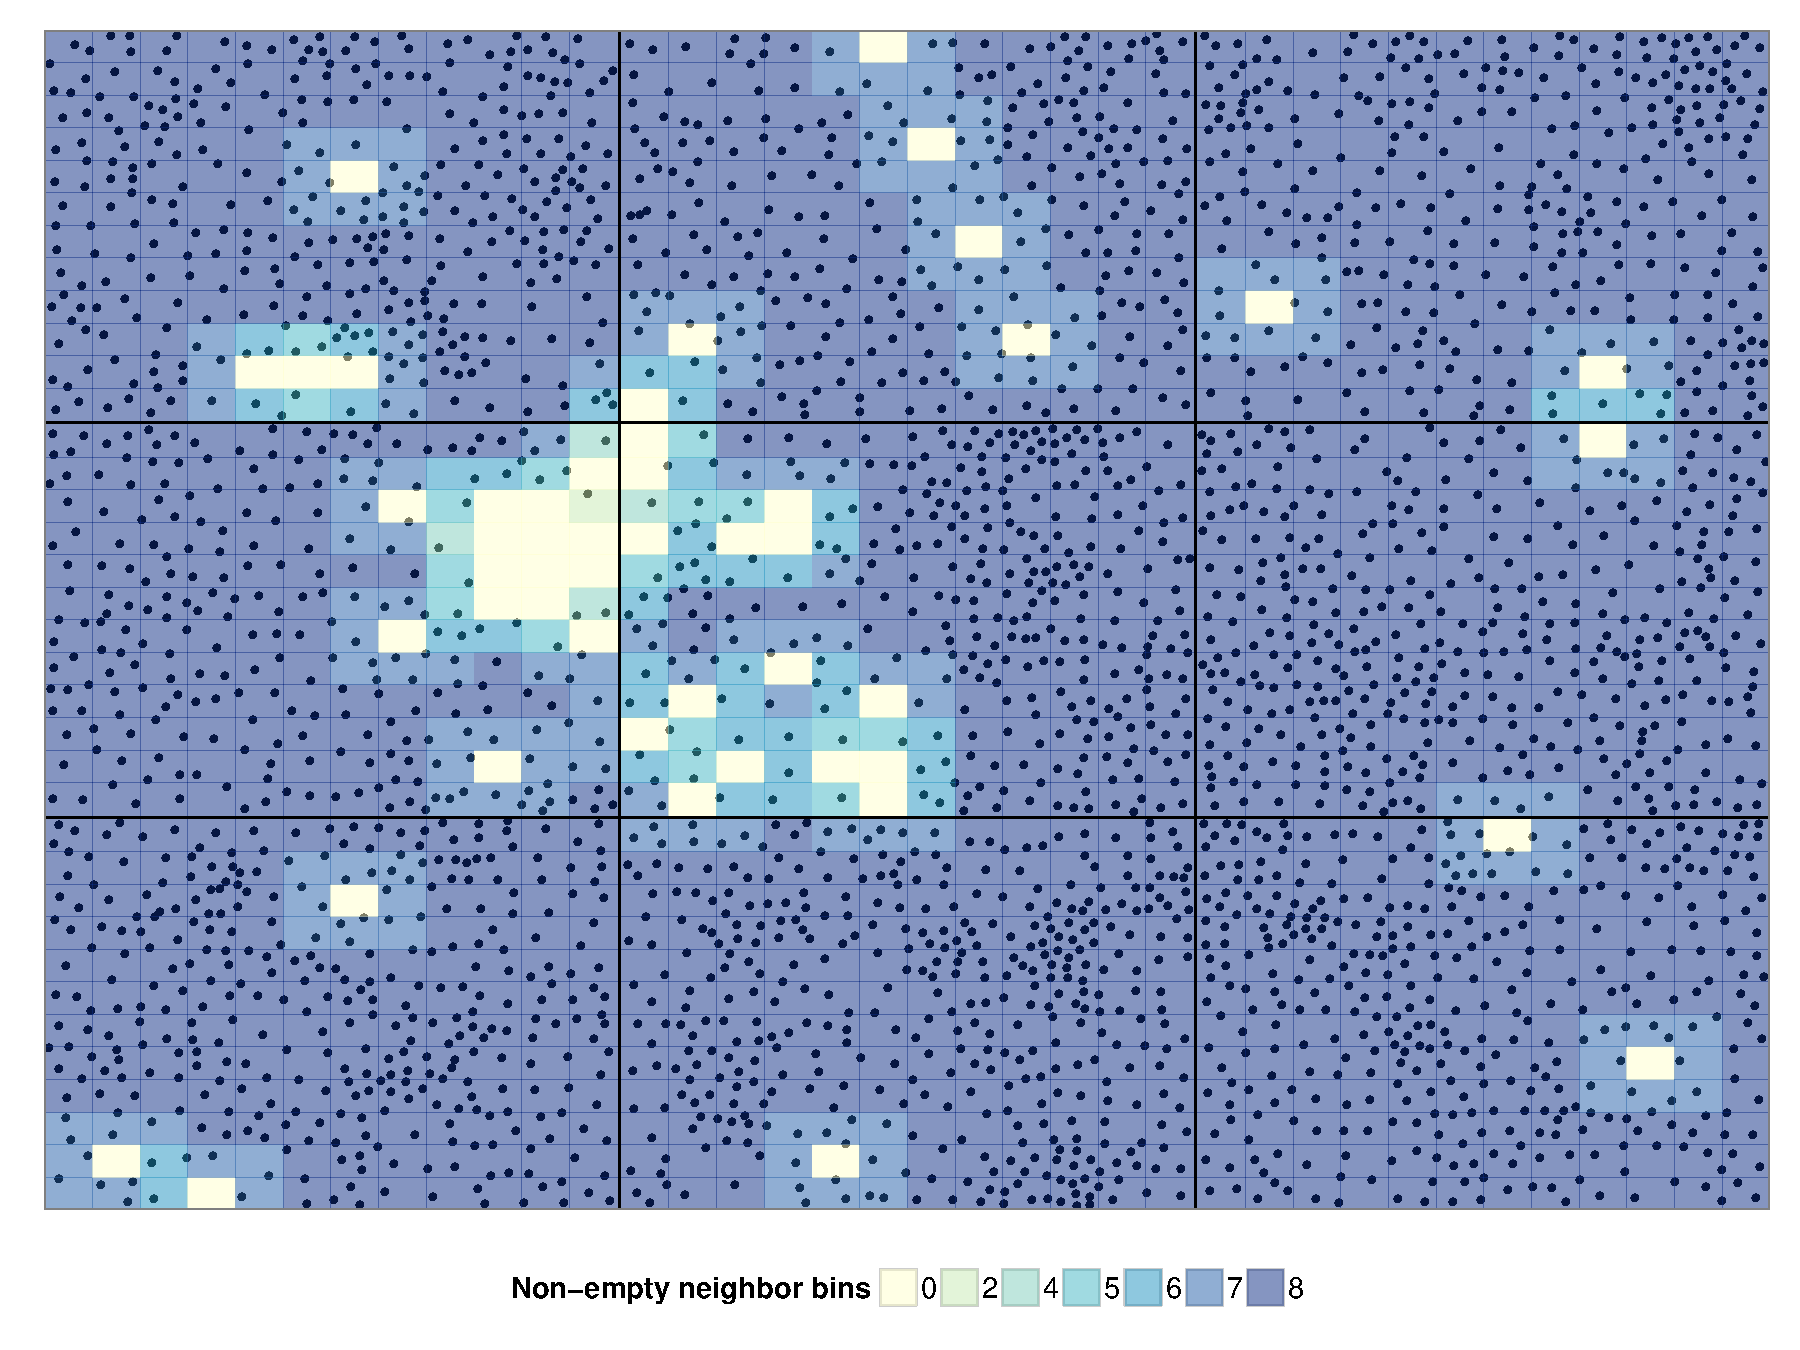
\includegraphics[width=\maxwidth]{figures/R/scf-intro/plot-scf-intro_plot-1} \caption[Visualization of cell colony edge detection by 2D binning.]{Cell colony edges are detected by 2D binning of cell center locations. Dots represent cell centers within the well H6 of plate J107-2C. Each of the nine images is segmented into 12 horizontal and 12 vertical sections yielding 144 tiles (1296 bins for the entire well). The tiles are colored according to the number of non-empty neighboring bins.}\label{fig:scf-intro_plot}
\end{figure}


\end{knitrout}


\label{ex:efficiency}
As proposed by \cite{Knapp2011} and \cite{Snijder2012}, the population context of each cell may significantly influence some morphological properties, as well as confound phenotypic information that is measured during feature extraction and therefore has to be accounted for. They propose several features that may act as proxies to characterize aspects of population context, one of which is whether a cell is located towards the border of a colony or is surrounded by cells in all directions. In order to approximate this information from location data, images are divided into 2-dimensional bins or facets and the number of cells per bin is counted. Cells that are located adjacent to one or more bins that are empty are considered edge cells and cells surrounded by non-empty bins are center cells. Figure \ref{fig:scf-intro_plot} visualizes the concept by color-coding facets according to the number of non-empty neighbors.

\begin{rlisting}{float=p}{Calculation of population context features as implemented by \citeauthor{Knapp2011}.}{In order to detect whether a cell is located towards the border of a colony or is surrounded by neighboring cells, each well is divided into 2-dimensional bins and the number of cells per bin is counted. As implemented by \citeauthor{Knapp2011}, all bins are iterated, each of the 8 possible directions (2 vertical, 2 horizontal and 4 diagonal) is checked for an empty neighbor and the corresponding binary value (at least one neighbor is empty) is saved to the current group of cells.}{edgepos}
\begin{knitrout}\footnotesize
\definecolor{shadecolor}{rgb}{0.969, 0.969, 0.969}\color{fgcolor}\begin{kframe}
\begin{alltt}
\hlstd{edgepos} \hlkwb{<-} \hlkwa{function}\hlstd{(}\hlkwc{x}\hlstd{,} \hlkwc{y}\hlstd{,} \hlkwc{img}\hlstd{,} \hlkwc{n}\hlstd{) \{}
  \hlstd{empty} \hlkwb{<-} \hlkwd{logical}\hlstd{()}
  \hlstd{xst} \hlkwb{<-} \hlstd{img[}\hlnum{1}\hlstd{]} \hlopt{/} \hlstd{n}
  \hlstd{yst} \hlkwb{<-} \hlstd{img[}\hlnum{2}\hlstd{]} \hlopt{/} \hlstd{n}
  \hlstd{sgrid} \hlkwb{<-} \hlkwd{matrix}\hlstd{(}\hlnum{0}\hlstd{,} \hlkwc{nrow}\hlstd{=n,} \hlkwc{ncol}\hlstd{=n)}
  \hlkwa{for} \hlstd{(i} \hlkwa{in} \hlnum{1}\hlopt{:}\hlstd{n) \{}
    \hlkwa{for} \hlstd{(j} \hlkwa{in} \hlnum{1}\hlopt{:}\hlstd{n) \{}
      \hlstd{ispos} \hlkwb{<-} \hlstd{(x} \hlopt{>} \hlstd{(i} \hlopt{-} \hlnum{1}\hlstd{)} \hlopt{*} \hlstd{xst)} \hlopt{&} \hlstd{(x} \hlopt{<=} \hlstd{(i} \hlopt{*} \hlstd{xst))} \hlopt{&}
               \hlstd{(y} \hlopt{>} \hlstd{(j} \hlopt{-} \hlnum{1}\hlstd{)} \hlopt{*} \hlstd{yst)} \hlopt{&} \hlstd{(y} \hlopt{<=} \hlstd{(j} \hlopt{*} \hlstd{yst))}
      \hlstd{sgrid[i, j]} \hlkwb{<-} \hlkwd{sum}\hlstd{(ispos)}
    \hlstd{\}}
  \hlstd{\}}

  \hlkwa{for} \hlstd{(i} \hlkwa{in} \hlnum{1}\hlopt{:}\hlstd{n) \{}
    \hlkwa{for} \hlstd{(j} \hlkwa{in} \hlnum{1}\hlopt{:}\hlstd{n) \{}
      \hlstd{ispos} \hlkwb{<-} \hlstd{(x} \hlopt{>} \hlstd{(i} \hlopt{-} \hlnum{1}\hlstd{)} \hlopt{*} \hlstd{xst)} \hlopt{&} \hlstd{(x} \hlopt{<=} \hlstd{(i} \hlopt{*} \hlstd{xst))} \hlopt{&}
               \hlstd{(y} \hlopt{>} \hlstd{(j} \hlopt{-} \hlnum{1}\hlstd{)} \hlopt{*} \hlstd{yst)} \hlopt{&} \hlstd{(y} \hlopt{<=} \hlstd{(j} \hlopt{*} \hlstd{yst))}
      \hlstd{isempty} \hlkwb{<-} \hlstd{F}
      \hlkwa{if} \hlstd{((i} \hlopt{>} \hlnum{1}\hlstd{)} \hlopt{&&} \hlstd{(j} \hlopt{>} \hlnum{1}\hlstd{)} \hlopt{&&} \hlstd{(sgrid[i} \hlopt{-} \hlnum{1}\hlstd{, j} \hlopt{-} \hlnum{1}\hlstd{]} \hlopt{==} \hlnum{0}\hlstd{))}
        \hlstd{isempty} \hlkwb{<-} \hlstd{T}
      \hlkwa{else if} \hlstd{((i} \hlopt{>} \hlnum{1}\hlstd{)} \hlopt{&&} \hlstd{(sgrid[i} \hlopt{-} \hlnum{1}\hlstd{, j]} \hlopt{==} \hlnum{0}\hlstd{))}
        \hlstd{isempty} \hlkwb{<-} \hlstd{T}
      \hlkwa{else if} \hlstd{((i} \hlopt{>} \hlnum{1}\hlstd{)} \hlopt{&&} \hlstd{(j} \hlopt{<} \hlstd{n)} \hlopt{&&} \hlstd{(sgrid[i} \hlopt{-} \hlnum{1}\hlstd{, j} \hlopt{+} \hlnum{1}\hlstd{]} \hlopt{==} \hlnum{0}\hlstd{))}
        \hlstd{isempty} \hlkwb{<-} \hlstd{T}
      \hlkwa{else if} \hlstd{((j} \hlopt{>} \hlnum{1}\hlstd{)} \hlopt{&&} \hlstd{(sgrid[i, j} \hlopt{-} \hlnum{1}\hlstd{]} \hlopt{==} \hlnum{0}\hlstd{))}
        \hlstd{isempty} \hlkwb{<-} \hlstd{T}
      \hlkwa{else if} \hlstd{((j} \hlopt{<} \hlstd{n)} \hlopt{&&} \hlstd{(sgrid[i, j} \hlopt{+} \hlnum{1}\hlstd{]} \hlopt{==} \hlnum{0}\hlstd{))}
        \hlstd{isempty} \hlkwb{<-} \hlstd{T}
      \hlkwa{else if} \hlstd{((i} \hlopt{<} \hlstd{n)} \hlopt{&&} \hlstd{(j} \hlopt{>} \hlnum{1}\hlstd{)} \hlopt{&&} \hlstd{(sgrid[i} \hlopt{+} \hlnum{1}\hlstd{, j} \hlopt{-} \hlnum{1}\hlstd{]} \hlopt{==} \hlnum{0}\hlstd{))}
        \hlstd{isempty} \hlkwb{<-} \hlstd{T}
      \hlkwa{else if} \hlstd{((i} \hlopt{<} \hlstd{n)} \hlopt{&&} \hlstd{(sgrid[i} \hlopt{+} \hlnum{1}\hlstd{, j]} \hlopt{==} \hlnum{0}\hlstd{))}
        \hlstd{isempty} \hlkwb{<-} \hlstd{T}
      \hlkwa{else if} \hlstd{((i} \hlopt{<} \hlstd{n)} \hlopt{&&} \hlstd{(j} \hlopt{<} \hlstd{n)} \hlopt{&&} \hlstd{(sgrid[i} \hlopt{+} \hlnum{1}\hlstd{, j} \hlopt{+} \hlnum{1}\hlstd{]} \hlopt{==} \hlnum{0}\hlstd{))}
        \hlstd{isempty} \hlkwb{<-} \hlstd{T}
      \hlstd{empty[ispos]} \hlkwb{<-} \hlstd{isempty}
    \hlstd{\}}
  \hlstd{\}}
  \hlkwd{return}\hlstd{(empty)}
\hlstd{\}}
\end{alltt}
\end{kframe}
\end{knitrout}

\end{rlisting}

Code listing \ref{lst:edgepos} constitutes an adaption of the implementation developed by \citeauthor{Knapp2011}, which is kindly provided as supplement to their publication. While iterating over all facets, only exploiting vectorization within facets and heavily relying on if-else logic, might be feasible when using datasets of the size the authors provide as demonstration material, combined with permanently storing the results, such an approach is impractical with datasets as produced by InfectX. Still, even for their datasets, the authors warn that:

\begin{quote}
These [population context feature] computations require considerable amounts of memory, and will take some time. This must be done for each of the input files, and will produce an output file containing the input data plus computed population features.
\end{quote}

\begin{rlisting}{float=p}{A more efficient implementation of calculating population context features, developed for singleCellFeatures.}{Due to the larger number of cells per well and the increase in image resolution as compared to data used in \cite{Knapp2011}, calculation of border/center population context features have to be carried out in a more efficient manner, which can be accomplished by fully vectorizing the problem.}{facetBorder}


\begin{rcode}
facetBorder <- function(x, y, img, facet) {
  facet.size <- img / facet
  # calculate facets (2d binning)
  x.bin <- ceiling(x / facet.size[1])
  y.bin <- ceiling(y / facet.size[2])
  # initialize empty grid/border matrices
  grid <- matrix(0, facet[2], facet[1])
  # calculate col-major grid index for each object
  index <- y.bin + (x.bin - 1) * facet[2]
  # summarize as counts
  counts <- table(index)
  # fill grid with counts
  grid[as.numeric(names(counts))] <- counts
  grid.res <- grid
  grid <- grid > 0
  # extend grid with a frame of ones
  grid.ext <- rbind(rep(1, (facet[1] + 2)),
                    cbind(rep(1, facet[2]), grid, rep(1, facet[2])),
                    rep(1, (facet[1] + 2)))
  # set up stencil
  row <- rep(rep(1:facet[2], facet[1]))
  col <- rep(1:facet[1], each=facet[2])
  colP1 <- col + 1
  colM1 <- col - 1
  rowP1 <- row + 1
  rowP2 <- row + 2
  nrowP <- facet[2] + 2
  stencil <- cbind(row   + colM1 * nrowP, # northwest neighbor
                   row   + col   * nrowP, # north neighbor
                   row   + colP1 * nrowP, # northeast neighbor
                   rowP1 + colP1 * nrowP, # west neighbor
                   rowP2 + colP1 * nrowP, # east neighbor
                   rowP2 + col   * nrowP, # southwest neighbor
                   rowP2 + colM1 * nrowP, # south neighbor
                   rowP1 + colM1 * nrowP) # southeast neighbor
  # apply stencil row-wise to grid
  border <- apply(stencil, 1, function(ind, mat) {
    return(sum(mat[ind]))
  }, as.numeric(grid.ext))
  # map col-major object index to border array
  return(border[index])
}
\end{rcode}


\end{rlisting}



\newcommand{\knitrScfRnaicellTotal}{\SI{2899.83}{\second}}
\newcommand{\knitrScfRnaicellEdgepos}{\SI{2892.67}{\second}}
\newcommand{\knitrScfRnaicellPercentage}{99.8\%}
\newcommand{\knitrScfRnaicellCellnoMean}{464}
\newcommand{\knitrScfRnaicellCellnoSd}{168}

An execution of the code, using the supplied exemplary dataset (number of cells per well: $\mu=\knitrScfRnaicellCellnoMean$, $\sigma=\knitrScfRnaicellCellnoSd$; 15 bins in x-direction and 15 bins in y-direction) reveals that of the \knitrScfRnaicellTotal\ spent on calculating population context features, \knitrScfRnaicellEdgepos\ (\knitrScfRnaicellPercentage\ of the total time) is spent on determining positions within colonies. This performance can be expected to deteriorate significantly, using InfectX data, due to a ten-fold increase in cell counts and more importantly a 3-fold rise in resolution in both x- and y direction. The surge in dataset size entails an increase in number of bins needed, to obtain sensible results (the example in figure \ref{fig:scf-intro_plot} is divided into 36 bins per dimension) and runtime scales as $\mathcal{O}(n^2)$ in number of bins per dimension.

Neither the high computational cost, and consequently not even storing the results, however are necessities, as demonstrated by a slightly optimized implementation (see listing \ref{lst:facetBorder}). Fully vectorizing the problem no longer requires the extensive use of if-else logic and due to R being an interpreted language, built for operating on vectors, such an approach can be expected to bring about compelling speed improvements. Vectorization is achieved by calculating the indices of the 8 neighboring bins for each facet and applying this stencil to the 2-dimensional matrix containing binary empty/non-empty information per bin. This efficiently yields the number of empty neighbors for each facet which then can be mapped to cells by their column-major grid indices. An additional advantage of the presented implementation is that the number of empty neighbors is obtained for free whereas the code proposed by \citeauthor{Knapp2011} would perform even worse if modified to produce this supplementary information, as the full set of if-statements has to be run to the end for each facet.



\newcommand{\knitrScfBenchmarkFacetMean}{\SI{7.77}{\milli\second}}
\newcommand{\knitrScfBenchmarkFacetSd}{\SI{2.69}{\milli\second}}
\newcommand{\knitrScfBenchmarkFacetTotal}{\SI{2.98} s}
\newcommand{\knitrScfBenchmarkEdgeMean}{\SI{515.85}{\milli\second}}
\newcommand{\knitrScfBenchmarkEdgeSd}{\SI{14.66}{\milli\second}}
\newcommand{\knitrScfBenchmarkEdgeTotal}{\SI{198.08}{\second}}
\newcommand{\knitrScfBenchmarkSpeedup}{66}

Benchmarking the two implementations reveals that a \knitrScfBenchmarkSpeedup -fold speedup is easily achievable only by completely vectorizing the problem. While the original code takes \knitrScfBenchmarkEdgeTotal\ per plate (384 iterations of the same well; $\mu=\knitrScfBenchmarkEdgeMean$, $\sigma=\knitrScfBenchmarkEdgeSd$; well H6 of plate J107-2C), total runtime is reduced to \knitrScfBenchmarkFacetTotal\ ($\mu=\knitrScfBenchmarkFacetMean$, $\sigma=\knitrScfBenchmarkFacetSd$, per well).

Such time-savings might not look that significant at first sight. But within the context of the available data, consequences of critical optimizations are of great value. First of all, interactive data analysis is sensitive to waiting times that exceed a few minutes and due to there not only being a single location feature to be analyzed, but rather 5--10, several minutes per feature are impractical. Moreover, if run-times can be sufficiently reduced, this makes it possible to run calculations on the fly instead of constantly saving results. Apart from the obvious downsides arising from storage overhead, management of result caches leads to practical issues whenever the workflow is under development and thus subject to constant change. Caches have to be invalidated and recomputed and the system overseeing these processes has to be made aware of changes, as well as understand where they apply.\footnote{On an anectotal note, Philip Karlton, a software engineer and former Netscape executive is quoted as saying: ``There are only two hard things in Computer Science: cache invalidation and naming things,'' corroborating the claim that it is desirable to avoid caching altogether whenever possible.} Furthermore, updating batches of data at once incurs substantial cost which might even be expended in vain if not all data is used before the next update triggers recomputation. Just in time generation of derived features is preferable over ahead of time calculation and the benefits clearly justify some optimization efforts.



\newcommand{\knitrScfFullPlateNSamp}{10}
\newcommand{\knitrScfFullPlateSampWell}{A1, A6, B1, B23, B9, E11, E14, I4, N20, P2}
\newcommand{\knitrScfFullPlateMyTime}{\SI{8.04}{\second}}
\newcommand{\knitrScfFullPlateRnaicellTime}{\SI{41.14}{\hour}}

When looking at runtimes of the original implementation obtained for benchmarking (\knitrScfBenchmarkEdgeTotal) and for a single execution on the supplied exemplary dataset (\knitrScfRnaicellEdgepos) side by side, a large discrepancy stands out. The two values are not directly comparable, as they are created with individual binning and differently sized datasets. But instead of explaining the divergence, these factors separate the two values even further, as the benchmarked time was obtained using a dataset roughly ten times larger and taking into account 6-fold more bins (225 versus 1296). Running the code of \citeauthor{Knapp2011} with InfectX data, as to be expected, takes significantly longer and determining cell position within colony for a single location feature over an entire plate is estimated to run for \knitrScfFullPlateRnaicellTime.\footnote{Due to the long running time, not all wells are processed, but \knitrScfFullPlateNSamp\ wells are randomly sampled and the mean per well is extrapolated to the full plate. The used wells are \knitrScfFullPlateSampWell\ of plate J107-2C. Moreover, it has to be emphasized once again, that the reported time-span corresponds only to the calculation of a single location feature, several of which are typically available.} The exact same results can be computed within \knitrScfFullPlateMyTime\ by the code integrated in singleCellFeatures through vectorization as discussed previously and by splitting the data into wells.

Listing \ref{lst:edgepos} does not entirely reproduce the code of \citeauthor{Knapp2011}, but constitutes a simplified version intended for highlighting the importance of vectorization and is adapted for comparison with the optimized variant. Originally, the nested for-loops iterating the bins (lines 6--12 and 14--37), are enclosed by an additional for-loop, iterating the wells. Data is stored as a large \mintinline{text}{data.frame} and all operations are performed on full-length vectors. The enormous number of comparisons resulting from this setup leads to serious performance issues, which are amplified when increasing the number of cells from $\sim 180000$ to $\sim 10^6$ per plate. Such observations, along with other considerations lead to development of a more sophisticated data structure for storing single cell feature data (see section \ref{sec:s3-objects}), which splits the data into smaller units and consequently eliminates constant comparisons against well indices for per-well operations.

The following sections discuss some design aspects and implementation issues of singleCellFeatures, beginning with data structures developed for representing single cell feature data, continuing with how data is acquired and locally cached, management of metadata and concluding with some tools for manipulating datasets as well as providing the data to third-party tools. This architectural overview is complemented by a more practical section in appendix \ref{ch:scf-manual}. For all coding, the style guide outlined in \cite{Wickham2014} was followed and \cite{Wickham2015} served as an invaluable reference, along with the extensive documentation supplied by \cite{RCoreTeam2015}. Package documentation is in-source with \mintinline{text}{.Rd} files generated by roxygen2 \citep{Wickham2015a}, which are accessible from within the R help system upon installation of the package.

\section{S3 Classes}
\label{sec:s3-objects}
\Gls{oop} in R can be achieved by any one of the three distinct object systems S3, S4 and \glspl{rc}. While the RC system resembles the \gls{oop} style most people coming from languages such as Java or C++ are familiar with, by implementing message-passing, some features such as mutability (in-place modification of objects) and pass-by-reference semantics violate common expectations of R users. S3 and S4 objects are built on the concept of generic function \gls{oop}, which does not associate methods with classes, but employs a special type of function, called a generic function, that is responsible for method dispatch. Of the two, S3 classes are more loosely organized, lacking the formal definitions of the S4 system which can describe both representation and (multiple) inheritance. Furthermore, S4 objects are capable of multiple dispatch and all code used for creating and manipulating S4 objects is not part of base R but supplied by the methods package, which introduces the new \mintinline{text}{@} operator, for accessing object slots.

Much base functionality in R is implemented using S3 classes, including lm and glm objects, the support for which has been available to R from its very beginning. The methods package for S4 objects is attached by default since version 1.7.0, but fewer packages make use of the newer syntax, some examples being the base package stats4 and CRAN packages Matrix and lme4. Bioconductor packages on the other hand are frequently designed on top of S4 classes. \Gls{rc} was only introduced with R 2.12 as part of the methods package and therefore currently does not enjoy widespread adoption. The limitations of S3 were found to be unproblematic for the planned feature set of singleCellFeatures and due to the attractive simplicity of this scheme, several objects are implemented as S3 classes.

\subsection{Metadata Objects}


\newcommand{\knitrScfMetadatNumCol}{44}
\newcommand{\knitrScfMetadatPlateQualityStat}{\mintinline{text}{UNKNOWN}, \mintinline{text}{GOOD}, \mintinline{text}{BAD} and \mintinline{text}{WARNING}}
\newcommand{\knitrScfMetadatPlateQualityFrac}{87\%}
\newcommand{\knitrScfMetadatPlateTypes}{\mintinline{text}{ScreeningPlate}, \mintinline{text}{CheckerBoard} and \mintinline{text}{MockPlate}}
\newcommand{\knitrScfMetadatSpaces}{\mintinline{text}{INFECTX} and \mintinline{text}{INFECTX_PUBLISHED}}
\newcommand{\knitrScfMetadatGeneset}{\mintinline{text}{Drug}, \mintinline{text}{Validation}, \mintinline{text}{MicroRNAome}, \mintinline{text}{Genome} and \mintinline{text}{Kinome}}
\newcommand{\knitrScfMetadatLibrary}{\mintinline{text}{Selleck}, \mintinline{text}{Ambion}, \mintinline{text}{Sigma}, \mintinline{text}{Dharmacon} and \mintinline{text}{Qiagen}}
\newcommand{\knitrScfMetadatWellQualityStat}{\mintinline{text}{UNKNOWN}, \mintinline{text}{WARNING} and \mintinline{text}{BAD}}
\newcommand{\knitrScfMetadatWellQualityFrac}{92\%}

\label{sec:metadata-objects}
Metadata is extracted from aggregate files (see section \ref{sec:aggregate-files}) and used to generate both plate-level and well-level metadata objects. These consist of key-value pairs stored as lists and accompany all plate-level and well-level data objects generated by singleCellFeatures. The R class attribute names are \mintinline{text}{PlateMeta data} or \mintinline{text}{WellMetadata} and both are associated with a superordinate object name \mintinline{text}{Metadata} in order to simplify method dispatch in cases where a function is able to operate on both object types. Table \ref{tab:plate-metadata} shows the 12 slots along with short descriptions that constitute a \mintinline{text}{PlateMetadata} object, while table \ref{tab:well-metadata} does the same for objects of type \mintinline{text}{WellMetadata} (20 key-value pairs in total). Several slots, namely \mintinline{text}{plate.barcode}, \mintinline{text}{plate.quality}, \mintinline{text}{experiment.name}, \mintinline{text}{experiment.pathogen}, \mintinline{text}{experiment.geneset} and \mintinline{text}{experiment.library}, are redundant and therefore only listed in table \ref{tab:plate-metadata}.

\renewcommand{\arraystretch}{1.5}
\setlength{\tabcolsep}{0.2em}
\begin{table}
  \centering
  \caption[Key-value pairs constituting the \mintinline{text}{PlateMetadata} structure.]{\mintinline{text}{PlateMetadata} structures consist of 12 key-value pairs intended to capture all relevant plate-wide metadata.}
  \label{tab:plate-metadata}
  \footnotesize
  \begin{tabular}{L{0.25\linewidth}L{0.7\linewidth}}
    Key name &
      Description \\
    \hline 
    \mintinline{text}{plate.barcode} &
      The unique identifier assigned to every plate, for example \mintinline{text}{KB02-1L}. \\
    \mintinline{text}{plate.quality} &
      Plate quality descriptors are \knitrScfMetadatPlateQualityStat, but currently most (\knitrScfMetadatPlateQualityFrac) are assigned the label \mintinline{text}{UNKNOWN}. \\
    \mintinline{text}{plate.type} &
      Possible values for plate type are \knitrScfMetadatPlateTypes\ and different types are characterized by their control layout. \\
    \mintinline{text}{experiment.space} &
      The first hierarchy level of data organization in openBIS. Current spaces are \knitrScfMetadatSpaces \\
    \mintinline{text}{experiment.group} &
      The group level is used to sort data according to pathogen (e.g. \mintinline{text}{ADENO_TEAM}). \\
    \mintinline{text}{experiment.name} &
      At the experiment level, data is grouped into screens. An example value is \mintinline{text}{ADENO-DP-K1}. \\
    \mintinline{text}{experiment.pathogen} &
      While the pathogen is already encoded in the openBIS hierarchy of InfectX, this is not necessarily so. In case of a different setup, the treatment applied to the screen can be saved separately. \\
    \mintinline{text}{experiment.geneset} &
      Different sets of genes are investigated throughout all screens and possible values are \knitrScfMetadatGeneset. \\
    \mintinline{text}{experiment.replicate} &
      Designates the replicate number of the current plate (see table \ref{tab:infectx-replicates}). \\
    \mintinline{text}{experiment.library} &
      Manufacturers that provide \gls{sirna} reagents to InfectX are \knitrScfMetadatLibrary. \\
    \mintinline{text}{experiment.batch} &
      Alphanumeric identifier for the batch in which the current plate was put through the wet-lab procedure. \\
    \mintinline{text}{counts.quantiles} &
      The lower and upper 5\% quantiles for cell counts over all 3456 images of the plate, determined in order to detect bad wells. \\
    \hline 
  \end{tabular}
\end{table}

\begin{table}
  \centering
  \caption[Metadata key-value pairs that make up \mintinline{text}{WellMetadata} objects.]{Analogously to \mintinline{text}{PlateMetadata} objects, \mintinline{text}{WellMetadata} classes consist of several key-value pairs. All slots that appear in both \mintinline{text}{Metadata} definitions (\mintinline{text}{plate.barcode}, \mintinline{text}{plate.quality}, \mintinline{text}{experiment.name}, \mintinline{text}{experiment.pathogen}, \mintinline{text}{experiment.geneset} and \mintinline{text}{experiment.library}) are excluded from this overview. Please refer to table \ref{tab:plate-metadata} for more information.}
  \label{tab:well-metadata}
  \footnotesize
  \begin{tabular}{L{0.25\linewidth}L{0.7\linewidth}}
    Key name &
      Description \\
    \hline 
    \mintinline{text}{well.row} &
      Capitalized alphabetic index of the current well row ($\in \{ A, B, \dotsc, P \}$). \\
    \mintinline{text}{well.col} &
      Integer-valued column index of the current well ($\in \{ 1, 2, \dotsc, 24 \}$). \\
    \mintinline{text}{well.index} &
      Well indices are calculated from row and column location and represent linearized, row-major well positions within plates ($\in \{ 1, 2, \allowbreak\dotsc, 384 \}$). \\
    \mintinline{text}{well.type} &
      Descriptor for the type of well, the most important of which include \mintinline{text}{SIRNA}, \mintinline{text}{POOLED_SIRNA} and \mintinline{text}{CONTROL}. \\
    \mintinline{text}{well.quality} &
     Possible values for this field are \knitrScfMetadatWellQualityStat, while most wells currently are set to \mintinline{text}{UNKNOWN} (\knitrScfMetadatWellQualityFrac). \\
    \mintinline{text}{gene.name} &
      Gene symbol corresponding to the targeted gene \citep{Gray2013}. \\
    \mintinline{text}{gene.id} &
      Entrez Gene ID of the targeted gene \citep{Maglott2011}. \\
    \mintinline{text}{sirna.name} &
      The \gls{sirna} catalog ID as specified by the manufacturer. \\
    \mintinline{text}{sirna.sequence} &
      Full sequence of the 5'-3' \gls{sirna} antisense (guide) strand added to the current well. \\
    \mintinline{text}{sirna.seed} &
      The seed sequence (nucleotides 2--9 from the 5' end) of the 5'-3' \gls{sirna} guide strand. \\
    \mintinline{text}{sirna.target} &
      Sense sequence of the \gls{sirna} target. \\
    \mintinline{text}{counts.cells} &
      The cell count of the current well. \\
    \mintinline{text}{counts.pathogen} &
      Count of recognized pathogen objects (in \textit{Bartonella} screens, the number of invasomes). \\
    \mintinline{text}{counts.infection} &
      Number of infected cells according to \gls{dtis}. \\
    \hline 
  \end{tabular}
\end{table}

Having metadata structures available alongside the objects holding single cell features facilitates manipulation of the data as all relevant information is bundled and does not have to be managed separately by the user. Furthermore, information stored in \mintinline{text}{well.type} can be used for normalization (sometimes it is desirable to only normalize non-control wells) and fields like \mintinline{text}{gene.name}, \mintinline{text}{gene.id} or \mintinline{text}{sirna.name} are used often for selecting the desired subset of data. The two slots \mintinline{text}{plate.quality} and especially \mintinline{text}{well.quality} hold promise for automatically discarding bad data, but current annotation levels leave much to be desired (\knitrScfMetadatPlateQualityFrac\ and \knitrScfMetadatWellQualityFrac, respectively, are labeled as \mintinline{text}{UNKNOWN}) due to the large amount of manual labor that is involved. Perhaps, if some form of automatic quality assessment is developed or if the results from focus detection are utilized to enhance data quality comments, these fields could be put to better use.

Originally, inspired by the cellHTS2 package, it was planned to use public databases for collecting further metadata, such as gene ontology, chromosomal location, gene function summaries and homology. The bioconductor package biomaRt \citep{Durinck2005,Durinck2009} can be used to query several web services, including Ensembl, Uniprot and Reactome with gene IDs \citep{Maglott2011} and retrieve gene annotations. Furthermore, \gls{sirna} sequences could be used for investigating \glspl{ote} and developing methods in order to correct for corresponding effects. Unfortunately, time constrains so far have prevented such ideas from being explored further.

\subsection{Data Objects}
Central to the presented R package are data structures that hold single cell feature data. Instead of just storing all data as a large \mintinline{text}{data.frame} as in RNAither, a more complex scheme was developed that represents the physical hierarchy of \gls{hts} datasets. This has both the advantage of presenting an intuitive structure of the data that can easily be navigated by the user, as well as efficiency benefits. Selecting cells from a well does not involve $10^6$ integer comparisons, but finding a slot in a list structure of length 384 (for consequences of the former approach, see the introductory example staring on page \pageref{ex:efficiency}).

Three types S3 objects represent the levels, data can be sorted by: 6 or 9 \mintinline{text}{ImageData} classes are assembled into a \mintinline{text}{WellData} object (which is additionally associated with a \mintinline{text}{WellMetadata} object) and 384 \mintinline{text}{WellData} structures, together with a \mintinline{text}{PlateMetadata} instance, compose a \mintinline{text}{PlateData} object. The respective collections of child objects are gathered in list structures named \mintinline{text}{data} (figure \ref{fig:scf-platedata} presents a visualization of this hierarchy). Name attributes are organized similarly as for metadata objects, with a superordinate tag \mintinline{text}{Data} assigned in addition to the individual descriptors, in order to be able to define functions that can be applied to all data objects in the same way.

The next logical level is the screen (\gls{sirna} library), but clustering several \mintinline{text}{PlateData} objects is infeasible with current hardware. As R keeps all loaded objects in memory and a plate consisting of \tilde 600 features on \tilde$10^6$ cells requires \tilde \SI{8}{\giga\byte}, only large memory systems could handle such data structures.\footnote{A large memory Euler node (a centralized \gls{hpc} resource provided by the ETH Z\"urich) was successfully used to operate on a collection of 8 \mintinline{text}{PlateData} objects for screen wide normalization trials, but the required \tilde \SI{220}{\giga\byte} of memory are currently not commonly available to desktop environments. Simply keeping the data in memory is not all that is required, as algorithmic overhead has to be factored in as well.}

\begin{figure}
  \centering
  \begin{tikzpicture}[%
    leaf/.style={grow=down,xshift=1em,anchor=west, edge from parent path={%
      (\tikzparentnode.south) |- (\tikzchildnode.west)}
    },
    level 1/.style={sibling distance=18em},
    level 2/.style={sibling distance=4em},
    level 3/.style={sibling distance=14em},
    level 4/.style={sibling distance=4em},
    vertex style/.style={
      draw=#1,
      thick,
      fill=#1!70,
      text=white,
      minimum width=1cm,
      minimum height=0.5cm,
      font=\footnotesize
    }
  ]
    \node[vertex style=Turquoise]{PlateData}
    [edge from parent fork down]
    child{node[vertex style=SeaGreen] {PlateMetadata}
      child[leaf,level distance=6ex] {%
        node[vertex style=BurntOrange]{plate.barcode}}
      child[leaf,level distance=12ex] {%
        node[vertex style=BurntOrange]{plate.quality}}
      child[leaf,level distance=18ex] {%
        node[vertex style=BurntOrange] {plate.type}}
      child[leaf,level distance=24ex] {%
        node[vertex style=BurntOrange] {\ldots}}
      child[leaf,level distance=30ex] {%
        node[vertex style=BurntOrange] {experiment.library}}
    }
    child {node[vertex style=MidnightBlue] {data}
      child {node[vertex style=Turquoise] {A1}}
      child {node[vertex style=Turquoise] {A2}
        child {node[vertex style=SeaGreen] {WellMetadata}
          child[leaf,level distance=6ex] {%
            node[vertex style=BurntOrange]{well.index}}
          child[leaf,level distance=12ex] {%
            node[vertex style=BurntOrange]{well.type}}
          child[leaf,level distance=18ex] {%
            node[vertex style=BurntOrange] {gene.name}}
          child[leaf,level distance=24ex] {%
            node[vertex style=BurntOrange] {\ldots}}
          child[leaf,level distance=30ex] {%
            node[vertex style=BurntOrange] {sirna.sequence}}
        }
        child {node[vertex style=MidnightBlue] {data}
          child {node[vertex style=Turquoise] {img\_11}
            child[leaf,level distance=6ex] {%
              node[vertex style=BurntOrange]{image.index}}
            child[leaf,level distance=12ex] {%
              node[vertex style=BurntOrange]{\ldots}}
            child[leaf,level distance=18ex] {%
              node[vertex style=MidnightBlue]{data.vec}}
            child[leaf,level distance=24ex] {%
              node[vertex style=MidnightBlue]{data.mat}}
            child[leaf,level distance=30ex] {%
              node[vertex style=MidnightBlue] {data.lst}}
          }
          child {node[vertex style=Turquoise] {img\_12}}
          child {node[vertex style=Turquoise] {\ldots}}
          child {node[vertex style=Turquoise] {img\_33}}
        }
      }
      child {node[vertex style=Turquoise] {\ldots}}
      child {node[vertex style=Turquoise] {P24}}
    };
  \end{tikzpicture}
  \caption[Data structure used for representing a complete plate of single cell data.]{Single cell data is organized according to the hierarchy imposed by \gls{hts} experiment design. Plates are divided into wells which are subdivided into images and Metadata objects (green) are attached at each level. Data objects provided by singleCellFeatures are in light blue and contain lists of subordinate objects (dark blue), while Metadata objects consist of key-value pairs (orange).}
  \label{fig:scf-platedata}
\end{figure}

The slots of \mintinline{text}{ImageData} objects are \mintinline{text}{plate} (barcode), \mintinline{text}{well.index} (linear, row-major, $\in \{ 1, 2, \dotsc, 384 \}$), \mintinline{text}{well.row} ($\in \{ A, B, \dotsc, P \}$), \mintinline{text}{well.col} ($\in \{ 1, 2, \dotsc, 24 \}$), \mintinline{text}{image.index} (linear, row-major, $\in \{ 1, 2, \dotsc, 6 \} \lor \{ 1, 2, \dotsc, 9 \}$, depending on number of imaging sites), \mintinline{text}{image.row} ($\in \{ 1, 2 \} \lor \{ 1, 2, 3 \}$, for 6 and 9 image wells, respectively), \mintinline{text}{image.col} ($\in \{ 1, 2, 3 \}$, independent on total number of images), \mintinline{text}{image.total} ($\in \{ 6, 9 \}$), \mintinline{text}{counts.quantiles} (the lower and upper 5\% quantiles of plate-wide, image level cell counts), \mintinline{text}{counts.cells}, \mintinline{text}{data.vec}, \mintinline{text}{data.mat} and \mintinline{text}{data.lst}.

Actual feature data is split according to dimensionality with respect to images or detected objects within images. Scalar-valued entities (such as object counts, minima, maxima, etc.) are saved into \mintinline{text}{data.vec} which represents the concatenated data as a vector-valued \mintinline{text}{data.frame} (in order to accommodate both numerical and character fields). Vector-valued features (the bulk of single cell data) are assembled into matrices, dependent on object counts, which are added to \mintinline{text}{data.mat}. While there are typically as many nuclei as cells, those features can be merged into the same matrix, but pathogen objects require their own data structure, as pathogen counts are different from cell counts. Furthermore, it may happen that cellular features come in different lengths due to segmentation errors. A final group of features is vector-valued per cell (matrix-valued per image) and is saved to the \mintinline{text}{data.lst} node. Currently, neighbor features are detected and converted to sparse adjacency matrices, using the Matrix package \citep{Bates2015}, while others, such as parent\slash child features, are represented by nested list structures.

One obvious advantage of the proposed data representation is storage efficiency for values that apply to groups of cells, such as plate and well-level metadata or all features of the \mintinline{text}{data.vec} group. When using a large matrix for all data, this information has to be duplicated \tilde 400 times at image level, \tilde 3500 times at well level and \tilde $10^6$ times at plate level, incurring significant storage overhead. This can be mitigated somewhat by using factors and the resulting structures can still be handled well by current hardware, but nonetheless, parsimony is desirable. For these reasons, metadata objects at image level were not developed, as they unnecessarily inflate object size, despite this breaking recursive symmetry. Instead, only the minimally necessary information for identifying the data source is attached at this level.

In retrospect, it is debatable whether spiting data into images is sensible or creates unnecessary computational overhead in traversing nested lists. At the time of original implementation it was unclear if all images could be treated equally and having this level of granularity available seemed important. With access to some practical experience in working with such structures, this feature may not be worth the complexity it entails. Splitting the data at well level, however has proven to be worthwhile.

\subsection{Auxiliary Objects}
\label{sec:auxiliary-objects}
Several additional S3 objects are implemented in an auxiliary capacity. Both \mintinline{text}{PlateLocation} and \mintinline{text}{WellLocation} classes serve to communicate the identity and location of datasets, while \mintinline{text}{PlateAggregate} and \mintinline{text}{MatData} objects are used for caching purposes.

Objects representing data locations are simple key-value lists that are instantiated with a barcode in case of \mintinline{text}{PlateLocation} or a barcode and a row\slash column specification for \mintinline{text}{WellLocation} objects. Subsequent population of slots \mintinline{text}{space}, \mintinline{text}{group} and \mintinline{text}{experiment} is performed by lookup of the information in the \mintinline{text}{plate.database} table (see section \ref{sec:plate-database}), which is an optimization measure necessary to speed up creation times severely hampered by retrieving the values from large aggregate files. The information contained in \mintinline{text}{DataLocation} (the class attribute to specify any of the two location types) objects uniquely specifies where the described dataset is located on openBIS and in local file-system cache and these classes are mainly used for unifying package-internal communication.

\begin{rlisting}{float=t}{Exemplary application of \mintinline{text}{DataLocation} objects.}{Mostly used for internal communication of dataset identity and location both within openBIS and the local file system, \mintinline{text}{DataLocation} objects simplify certain tasks such as lookup of cache files.}{getCacheFilenameData}


\begin{rcode}

getCacheFilenameData <- function(x) {
  UseMethod("getCacheFilenameData", x)
}

getCacheFilenameData.WellLocation <- function(x) {
  config <- configGet()
  name <- paste0(x$plate, "_", x$row, x$col, "_sc_all.rds")
  path <- paste(config$dataStorage$dataDir, x$space, x$group, 
    x$experiment, x$plate, "WellData", name, sep = "/")
  return(path)
}

getCacheFilenameData.PlateLocation <- function(x) {
  config <- configGet()
  name <- paste0(x$plate, "_sc_all.rds")
  path <- paste(config$dataStorage$dataDir, x$space, x$group, 
    x$experiment, x$plate, name, sep = "/")
  return(path)
}

getCacheFilenameData.default <- function(x) {
  stop("can only deal with DataLocation (PlateLocation/WellLocation) objects.")
}

\end{rcode}


\end{rlisting}

Before introduction of \mintinline{text}{DataLocation} objects, a fair amount of redundant code was necessary for simple tasks such as saving or retrieving cache files. Identity of datasets was mostly specified by passing plate barcodes\slash experiment names and from that information, paths were assembled. Cumbersome casting of letter case, splitting strings to separate pathogen from library and adding setup-specific strings (such as \mintinline{text}{_TEAM}, which added as suffix to an all caps pathogen name yields the openBIS project name) to generate the appropriate values determining local file paths, as well as performance issues due to constant lookups of the same information can altogether be avoided by using specialized objects containing all neccessary information. Furthermore, the S3 method dispatch system can be put to use for specifying different behavior dependent on the object that is used as function argument. For a small illustration of such as use case, see code listing \ref{lst:getCacheFilenameData}.

The two remaining auxiliary objects are both used for caching purposes. Due to the narrow purpose of \mintinline{text}{DataLocation} a lookup table containing all required information can be created, that remains small enough to be loaded quickly. This is not possible for creating metadata objects, as most aggregate file columns are required for this process. In order to prevent repeated loading of these large files (100--\SI{200}{\mega\byte}, plate-level excerpts are cached as \mintinline{text}{PlateAggregate} objects whenever first accessed. The resulting files are small (\tilde \SI{100}{\kilo\byte}) and can be attached quickly. The data structure is simple, containing of two slots \mintinline{text}{plate} and \mintinline{text}{data}, the former holding a \mintinline{text}{PlateLocation} object and the latter a \mintinline{text}{data.frame} storing the relevant 384 rows of the corresponding aggregate file.

Finally, \mintinline{text}{MatData} is a type of \mintinline{text}{Data} object, that can be though of as a precursor to a \mintinline{text}{PlateData} object. The reason for its existence lies in the dynamic nature of this project. Many parts of singleCellFeatures evolved considerably and constant change poses problems for cached data structures. Originally, \mintinline{text}{PlateData} objects themselves were saved to the local file system but whenever their implementation was modified, all instances had to be invalidated and rebuilt (which initially took \tilde\SI{45}{\minute} per plate). In order to improve the situation, not \mintinline{text}{PlateData} objects are written to disk, but a data structure that holds all MATLAB feature data in a large nested list, as it is imported into R. Two slots are available to a \mintinline{text}{MatData} object, one called \mintinline{text}{meta} and intended for holding a \mintinline{text}{PlateMetadata} object and the oder is named \mintinline{text}{data} and stores all single cell features.

This successfully addresses the outlined problem, since the raw data will not change frequently (it still can occur that for example new features are developed\footnote{The system is build with a fair amount of flexibility, as there are methods available for adding new features to existing \mintinline{text}{MatData} structures, including automatic invalidation of downstream well caches. Therefore, extraction of new features does not require the rebuild of whole \mintinline{text}{MatData} objects.}, or better segmentation is employed), but introduces a new issue: build up of \mintinline{text}{PlateData} objects from \mintinline{text}{MatData} has to be reasonably fast due to this being the first step in every interactive session. Some aspects of how this is achieved is discussed in section \ref{sec:data-access}.

None of these auxiliary data structures are implemented as S3 objects for simply defining a set of fields, but much rather for their capability of using generic functions that specify how a specific procedure is applied to the different object variants. While this by itself is not an indispensable feature, as one could simple choose different but related names for the set of procedures, it is greatly appreciated for helping to organize code into functional units. Furthermore, this reduces the amount of redundant code by allowing the same function name to be applied in different contexts (for examples of this, see listings \ref{lst:feature-compat} and \ref{lst:convert}).

\section{Data Access}
\label{sec:data-access}
The core capability of singleCellFeatures is seamlessly providing the user with single cell data and doing this within time-frames that are suitable for interactive usage. As already discussed in the introduction to this chapter, some form of local caching is necessary to to meet these goals, as downloading data from openBIS and especially loading a large number of MATLAB \mintinline{text}{.mat} files into R takes a considerable amount of time.

Several tools were developed, beginning with search capabilities in order to locate the datasets of interest, followed by a set of functions that sort the queried data into units such that fetching is as economical as possible thusly minimizes waiting times and trigger retrieval from a multilevel cache system. All of this is handled in the background with no user intervention required. The following short example is intended for highlighting the effectiveness of the proposed system.



\begin{rflow}
time <- system.time({
  plates <- findPlates(contents="MTOR",
                       experiments="brucella-du-k[12]")
  wells  <- findWells(contents=c("MTOR", "SCRAMBLED"),
                      plates=unlist(plates))
  data   <- getSingleCellData(wells)})
\end{rflow}

\newcommand{\knitrScfFindGetDemoTime}{\SI{44}{\second}}
\newcommand{\knitrScfFindGetDemoSize}{\SI{1.22}{\giga\byte}}
\newcommand{\knitrScfFindGetDemoLengthW}{104}
\newcommand{\knitrScfFindGetDemoLengthP}{8}


In order to retrieve data from all plates containing wells with \gls{sirna} directed against \gls{mtor}, a list of \mintinline{text}{PlateLocations} is generated by \mintinline{text}{findPlates}. Acting on that structure, \mintinline{text}{findWells} selects all wells containing scrambled control \gls{sirna}, as well as \gls{mtor} knockdown wells and returns a list of \mintinline{text}{WellLocations}. Retrieving the resulting \knitrScfFindGetDemoLengthW\ wells, spread over \knitrScfFindGetDemoLengthP\ plates (\knitrScfFindGetDemoSize\ of data), is accomplished within \knitrScfFindGetDemoTime. In this case, all well data was read from cache, but apart from an increase in runtime, the same code snippet can be used irrespective of local cache state and will produce identical results. Figuring out how to proceed most efficiently in any case is handled by singleCellFeatures.

\begin{figure}
  \centering
  \begin{tikzpicture}[%
    decision style/.style={%
      diamond, draw=#1, on grid, thick, fill=#1!70, inner sep=2pt, aspect=2, 
      text=white, text width=5em, text centered, font=\footnotesize
    },
    block style/.style={%
      rectangle, draw=#1, on grid, thick, fill=#1!70, rounded corners,
      minimum height=3em, inner sep=4pt, minimum width=7em, text=white,
      text width=5em, text centered, font=\footnotesize
    },
    cloud style/.style={%
      ellipse, draw=#1, on grid, thick, fill=#1!70, minimum height=3em,
      minimum width=6em, inner sep=2pt, text=white, text width=5em,
      text centered, font=\footnotesize
    },
    line style/.style={%
      draw, -latex'
    }
  ]
  % Place nodes
  \node [cloud style=SeaGreen] (dataLoc) {%
    List of \mintinline{text}{DataLocation} objects};
  \node [block style=SeaGreen, left = 3.75cm of dataLoc] (find) {%
    Find data (wells, plates)};
  \node [block style=Turquoise, right = 3.75cm of dataLoc] (sort) {%
    Sort \mintinline{text}{DataLocations} by plate};
  \node [decision style=Turquoise, below = 2.5cm of dataLoc] (onlyWell) {%
    Were only cached wells requested?};
  \node [cloud style=Turquoise, below = 2.5cm of find] (done) {%
    Add to results};
  \node [block style=Turquoise, below = 2.5cm of sort] (iterate) {%
    Iterate plates};
  \node [decision style=BurntOrange, below = 2.5cm of iterate] (plateCache) {%
    Does \mintinline{text}{MatData} cache exist?};
  \node [decision style=BurntOrange, below = 2.5cm of plateCache] (matFiles) {%
    Are \mintinline{text}{.mat} files present?};
  \node [block style=BurntOrange, below = 2.5cm of matFiles] (download) {%
    Download data from openBIS};
  \node [block style=BurntOrange, left = 3.75cm of matFiles] (import) {%
    Import \mintinline{text}{.mat} data into R, save
    \mintinline{text}{MatData} cache};
  \node [cloud style=BurntOrange, left = 3.75cm of plateCache] (plateData) {%
    Build \mintinline{text}{PlateData} object};
  \node [decision style=Turquoise, left = 3.75cm of plateData] (wellReq) {%
    Were any uncached wells requested?};
  \node [block style=Turquoise, left = 3.75cm of import] (wellCache) {%
    Extract wells, cache \mintinline{text}{WellData} objects};
  % Draw edges
  \path [line style] (find) -- (dataLoc);
  \path [line style] (dataLoc) -- (sort);
  \path [line style] (sort) -- (iterate);
  \path [line style] (iterate) -- (onlyWell);
  \path [line style] (done.north) |-(0cm,-1.25cm)-| (iterate.north);
  \path [line style] (onlyWell) |-(0cm,-3.75cm)-| node[pos=0.25,above]{%
    no}(plateCache);
  \path [line style] (onlyWell) -- node[above]{yes}(done);
  \path [line style] (plateCache) -- node[right]{no}(matFiles);
  \path [line style] (matFiles) -- node[right]{no}(download);
  \path [line style] (download) -| (import);
  \path [line style] (matFiles) -- node[above]{yes}(import);
  \path [line style] (plateCache) -- node[above]{yes}(plateData);
  \path [line style] (import) -- (plateData);
  \path [line style] (plateData) -- (wellReq);
  \path [line style] (wellReq) -- node[right]{no}(done);
  \path [line style] (wellReq) -- node[right]{yes}(wellCache);
  \path [line style] (wellCache.west) |-(-5.75cm,-7.5cm)|- (done.west);
  \end{tikzpicture}
  \caption[Simplified view of the steps involved in loading single cell data.]{Three separate procedures are involved in loading single cell data. First, the functions \mintinline{text}{findPlates} and \mintinline{text}{findWells} can be used to run queries and retrieve a list of \mintinline{text}{DataLocation} objects (green) which is passed on to the function \mintinline{text}{getSingleCellData} (blue). Data requests are sorted according to plate and the list of plates is iterated. Dependent on request and availability of caches, \mintinline{text}{DataLocation} objects are assembled (orange) and returned to the calling function. This diagram represents a simplified view and several additional features complicate the underlying logic. For example, only a subset of features can be requested, in which case, writing of well caches has to be handled separately. Furthermore, checks for data completeness and consistency are employed that may alter the outlined execution path and mechanisms for recovery from unsuccessful imports are also in place but not shown.}
  \label{fig:scf-data-import}
\end{figure}

The most important steps in this procedure are visualized by figure \ref{fig:scf-data-import}. For sake of brevity, several aspects that complicate the logic underlying data access are omitted from the diagram. Some examples include recovery from failed downloads or imports, checks for completeness and consistency of the fetched data, issues involving metadata and the ability to only retrieve a subset of single cell feature, which requires special attention to down-stream caching. Color coding corresponds to the functional units searching (green), ordering the query and executing individual fetches (blue), as well as building the required data structures (orange). 

Searching relies on search indexes that are stored as a single plate database and pathogen specific well databases in order to be carried out quickly and economically. These lookup tables are derived from metadata contained in aggregate files and are described in detail in sections \ref{sec:plate-database} and \ref{sec:aggregate-files}. Further information regarding search functionality, such as arguments recognized by the two functions and how exactly search strings are matched is available in section \ref{sec:dataset-search}. The resulting list of \mintinline{text}{DataLocation} objects is passed to the function \mintinline{text}{getSingleCellData}, which acts as a conduit between searches and fetches.

The inquiry has to be ordered plate wise, in case uncached wells are sought from different plates. If such requests are carried out interleaved, large plate caches are read redundantly, entailing unnecessary overhead. The plates involved are iterated and it is checked if only cached wells are requested, in which case they are read from disk and added to the result structure. If uncached wells need to be made available or a complete plate is solicited, the corresponding \mintinline{text}{PlateData} object has to be built, the particularities which (orange nodes in figure \ref{fig:scf-data-import}) will be explored throughout the following subsections. Finally, if only wells were requested, they are extracted from the \mintinline{text}{PlateData} structure and added to the list of results and if the complete plate data is of interest it is returned as-is.

Green and blue nodes in figure \ref{fig:scf-data-import} can be bypassed entirely if only few single data structures are of interest. Instantiating a single \mintinline{text}{WellData} object, for example, that is not cached, will trigger the build up of a \mintinline{text}{PlateData} structure, followed by the extraction of that well. This, of course is inefficient, if multiple wells of the same plate are needed, as the plate structure is repeatedly created and discarded. In such a scenario, the functions described above can be utilized, or \mintinline{text}{PlateData} object itself can be instantiated, following well extraction initiated by the user (via the functionality provided by \mintinline{text}{extractWells}). These concepts are best illustrated by a quick example:

\label{ex:dataobject-instantiation}
\begin{rflow}
# set up a few data location objects
well.locs <- list(WellLocation("J107-2C", "H", 6),
                  WellLocation("J107-2C", "G", 23))
# inefficient if well caches do not exist, as the corresponding plate
# cache will be loaded twice, otherwise quickest option
wells <- lapply(well.locs, WellData)
# best if plate data already loaded or well caches inexistent
plate <- PlateData(convertToPlateLocation(well.locs[[1]]))
wells <- extractWells(plate, well.locs, keep.plate=FALSE)
# singleCellFeatures figures out how to proceed optimally
wells <- getSingleCellData(well.locs)
\end{rflow}

The remainder of the current section will focus on topics revolving around data provisioning itself, involving data acquisition, caching and build-up of \mintinline{text}{PlateData} structures (orange nodes in figure \ref{fig:scf-data-import}).

\subsection{Data Download}
Fetching data from openBIS, in case neither corresponding MATLAB files, nor a \mintinline{text}{MatData} cache file exists,\footnote{A third scenario that will trigger data download is manual override. If, for some reason cached data gets corrupted, or if a newer version of a dataset is available on openBIS, the user can choose to re-download individual plates. In addition, removal of all caches can be triggered, but for most circumstances this presents too drastic a measure.} is performed by issuing a system call and running the Java command line executable that is supplied with openBIS. Currently, three different types of files can be downloaded

\begin{center}
\mintinline{text}{HCS_ANALYSIS_CELL_FEATURES_CC_MAT}
\mintinline{text}{HCS_ANALYSIS_CELL_DECTREECLASSIFIER_MAT}
\mintinline{text}{HCS_ANALYSIS_CELL_THRESHOLDEDINFECTIONSCORING_MAT}
\end{center}

and the downloading routine can be run in two different modes, one targeting single cell feature files (filtering for the first file type, \mintinline{text}{FEATURES_CC}), while the other is intended for fetching \gls{dtis} results and prefers \mintinline{text}{DECTREECLASSIFIER} but falls back to \mintinline{text}{THRESHOLDEDINFECTIONSCORING} when the former is unavailable. The two types of infection scores represent two generations of \gls{dtis} procedures (distinct from \gls{svm} based scoring which were used before) and while the newer files are available for many plates, there are some that have not yet been updated. The downloaded set of files can further be refined by supplying a regular expression that is passed on the Java utility, but this will prevent downstream caches from being created (at well level) and create a plate level cache that is incomplete (can be completed without re-fetching the already downloaded data). All \mintinline{text}{.mat} files are saved to a temporary location within the directory structure managed by singleCellFeatures.

\subsection{Data Import}
Following completion of all download tasks, the resulting list of files is read into R using the function \mintinline{text}{readMat} of R.matlab \citep{Bengtsson2015}. For unknown reasons this function sometimes fails to import a file,\footnote{Failure is rare and does not seem to be dependent on file-level corruption, as retrying the same file usually resolves the problem. Furthermore, so far, no patterns could be made out, in that affected files appear to be somewhat random. The issue was not investigated further as a pragmatic approach resolved the problem.} which is caught, the affected file is saved into a special directory and import is allowed to continue. Due to this being the most time-consuming step in data provisioning, the results are stored as incomplete \mintinline{text}{MatData} caches and functionality for completing the data structure as opposed to entirely rebuilding it, are available. The function \mintinline{text}{rebuildCache} automatically retries files that failed during initial import and is capable of re-downloading individual features from openBIS that are missing from the \mintinline{text}{MatData} structure without user intervention.\footnote{The necessity for re-downloading is distinct from re-importing. While the latter arises from the possibility of failed reads of \mintinline{text}{.mat} files, the former is a consequence of problems that surround the openBIS hardware implementation of InfectX. Due to infrastructure work during much of the time of this project, it could not be guaranteed that the downloaded set of features comprises the full set of available features. This issue is remedied by checking for completeness of the local feature-set after build-up of a \mintinline{text}{MatData} structure in combination with semi-autonomous and cheap addition of individual features in case some are found to be missing.}\footnote{\label{fn:feat-check}Missingness currently is determined by comparison to a pathogen specific list of features. While being a very simple approach, it may lead to false positives (features that are indicated to be missing but do not exist), as well as false negatives (features that are present but indicated to be superfluous), as the set of features is not only pathogen specific, but also dependent on the analysis pipeline version. Improvements to this scheme are feasible (for example querying openBIS metadata directly or creating screen level lists) but not implemented due to time constraints and acceptable performance of the current system (see section \ref{sec:feature-lists} for more information).} Furthermore, the location of manually downloaded files can be specified in order for them to be added to the data structure and down stream caches of \mintinline{text}{WellData} structures are automatically removed whenever the \mintinline{text}{MatData} object is rewritten, as they are no longer valid.

Upon successful assembly of a \mintinline{text}{MatData} object, it is written to disk. Due to the large size of these objects (a typical plate is \tilde \SI{8}{\giga\byte} in size) good and efficient compression is essential both from a perspective of economically utilizing storage space, as well as from the viewpoint of time consumption. All major compression programs (bzip2, gzip, xz and zip) offer a parameter to adjust the speed\slash file size trade-off (usually an integer between 1 and 9) but a high compression ratio entails significant performance penalties. For storage of \mintinline{text}{MatData} objects, smallest file sizes were obtained using xz with flags \mintinline{text}{-9} or \mintinline{text}{-e}, which were on the order of 1--\SI{1.5}{\giga\byte}.

\begin{rlisting}{float=t}{Wrapper around pigz in order to speed up compression times for \mintinline{text}{MatData} objects.}{Compression with base library functions is not sufficiently performant, leading to the implementation of functions wrapping around \mintinline{text}{readRDS}\slash\mintinline{text}{saveRDS} that are capable of exploiting parallelized compression algorithms. The best overall compromise between compression\slash decompression speed and file size was obtained with pigz at compression level setting \mintinline{text}{-9}.}{pigz}


\begin{rcode}

saveRDSMC <- function(object, file, threads = getNumCores()) {
  message("using ", threads, " threads for compression.")
  con <- pipe(paste0("pigz -p ", threads, " -9 -f > ", file), "wb")
  saveRDS(object, file = con)
  on.exit(if (exists("con")) close(con))
}

readRDSMC <- function(file) {
  con <- pipe(paste0("pigz -d -k -c ", file))
  object <- tryCatch({
    readRDS(file = con)
  }, error = function(err) {
    stop("could not read file\n", file, ":\n", err)
  }, finally = {
    if (exists("con")) close(con)
  })
  return(object)
}

\end{rcode}


\end{rlisting}

While slightly longer compression times might be worth the savings in storage space, the time required for decompression is critical, as it will be the first step of every analysis procedure. Unfortunately, retrieval of highly compressed xz files is too slow for this application. Moreover, parallelized implementations lbzip2, p7zip, PBZIP2, pigz and xz with option \mintinline{text}{-T} were tested and and the best overall compromise is achieved using pigz with option \mintinline{text}{-9}, as shown in code listing \ref{lst:pigz}. Typical file sizes using this procedure are 1.5--\SI{2}{\giga\byte} for a complete \mintinline{text}{MatData} object and compression takes around \SI{10}{\minute}.

After the plate cache file is written, all successfully read \mintinline{text}{.mat} files are deleted, while failed files are kept for subsequently re-attempting import. Whenever the cache is read from disk, it is checked for feature completeness and the user is informed of deviations from the expected state. Due to the current implementation this is prone to some erroneous warnings especially for older plates that have not been updated to the newest feature extraction procedures (see footnote \ref{fn:feat-check}), upon which reporting is based.

\subsection{Creation of \mintinline{text}{Data} Structures}
Irrespective of whether a given plate is already in cache or is requested for the first time, every \mintinline{text}{PlateData} structure is built from a \mintinline{text}{MatData} object. As mentioned in section \ref{sec:auxiliary-objects}, the motivation behind this is creating independence between the implementation of \mintinline{text}{PlateData} structures and the data itself and consequently no longer invalidating cached plate data by making changes to its representation. This requires the conversion of \mintinline{text}{MatData} into \mintinline{text}{PlateData} to be reasonably fast and much effort was invested in reducing the amount of time needed for this step.

The critical section in this process is creating the individual \mintinline{text}{ImageData} objects from the list structure resembling how single cell features are stored by CellProfiler. Listing \ref{lst:splitImages} displays a segment of the code involved and while it might appear cluttered at first sight and the context of many variables is unclear, it is reproduced in order to highlight some important aspects. At this point in execution, among other things, the features have been sorted into groups according to their dimensions. Every feature is represented by a list containing as many slots as there are images on a plate and each slot holds a further list structure, the length of which is used for sorting. Single element objects are grouped into \mintinline{text}{vec} and handled by the code in lines 4--10, lists with multiple scalar elements are added to \mintinline{text}{mat} and treated by lines 12--29, while entries that constitute of a further nesting level are stored in \mintinline{text}{lst} and dealt with by lines 31--73. With this structure established, the outermost \mintinline{text}{apply}-type function sets up an index that moves through all lists simultaneously and in each step, the data corresponding to the given image is extracted and molded into an \mintinline{text}{ImageData} structure.

\afterpage{\clearpage\begin{rlisting}{enlarge bottom finally by=0.75cm, nofloat}{An excerpt of the code resposible for converting \mintinline{text}{MatData} into \mintinline{text}{PlateData} objects.}{Due to the heterogeneity of InfectX datasets, build up of \mintinline{text}{PlateData} structure is fairly involved, as many edge cases have to be handled. Moreover, every instantiation of a \mintinline{text}{PlateData} object is preceded by the conversion from a \mintinline{text}{MatData} structure, requiring quick turnover. This code excerpt shows the section responsible for building \mintinline{text}{ImageData} objects from a nested list structure akin to what is produced by CellProfiler, by moving through all lists simultaneously and in building an image data object in every iteration. The three sections \mintinline{text}{vec}, \mintinline{text}{mat} and \mintinline{text}{lst} correspond to different types of features that are grouped according to their dimensions.}{splitImages}
\begin{rcode}
data$data <- plyr::llply(1:tot.nimgs, function(ind, data, name,
                                               n.imgs, quants, counts) {
  if(length(data$vec) > 0) {
    vec <- lapply(data$vec, function(group, ind) {
      return(data.frame(lapply(group, function(feature, i) {
        return(feature[[i]])
      }, ind), stringsAsFactors=FALSE, check.names=FALSE, check.rows=FALSE))
    }, ind)
  } else {
    vec <- NULL
  }
  if(length(data$mat) > 0) {
    mat <- lapply(data$mat, function(group, ind) {
      n.rows <- length(group[[1]][[ind]])
      grp <- vapply(group, function(feature, i) {
        return(unlist(feature[i]))
      }, double(n.rows), ind)
      names <- colnames(grp)
      if(is.null(names)) names <- names(grp)
      n.cols <- length(names)
      dim(grp) <- c(n.rows, n.cols)
      colnames(grp) <- names
      rownames(grp) <- NULL
      return(grp)
    }, ind)
  } else {
    mat <- NULL
  }
  if(length(data$lst) > 0) {
    lst <- mapply(function(group, gname, ind) {
      if(gname == "IdentityOfNeighbors") {
        return(lapply(group, function(feature, i) {
          # build sparse adjacency matrices
          l <- length(feature[[i]])
          if(l > 1) {
            p <- c(0, cumsum(sapply(feature[[i]],
                             function(x) length(x[[1]]))))
            j <- unlist(feature[[i]])
            return(sparseMatrix(j=j, p=p, dims=c(l, l)))
          } else return(NULL)
        }, ind))
      } else if(gname == "PercentTouchingNeighbors") {
        return(lapply(group, function(feature, i) {
          if(length(feature[[i]]) > 1) return(unlist(feature[[i]]))
          else return(NULL)
        }, ind))
      } else {
        return(lapply(group, function(feature, i) return(feature[i]), ind))
      }
    }, data$lst, names(data$lst), list(ind=ind), SIMPLIFY=FALSE)
  } else {
    lst <- NULL
  }
  if(!is.null(lst$PercentTouchingNeighbors) & 
     !is.null(lst$IdentityOfNeighbors)) {
    lst$PercentTouchingNeighbors <- mapply(function(feat, fname, mats) {
      object <- unlist(strsplit(fname, 
                                "Neighbors.PercentTouchingNeighbors"))[2]
      mat <- mats[[grep(paste0("Neighbors.IdentityOfNeighbors", object),
                        names(mats))]]
      if(is.null(mat)) {
        return(feat)
      } else {
        return(sparseMatrix(j=mat@i, p=mat@p, x=feat, dims=dim(mat),
               index1=FALSE))
      }
    }, lst$PercentTouchingNeighbors, names(lst$PercentTouchingNeighbors),
       list(mats=lst$IdentityOfNeighbors), SIMPLIFY = FALSE)
  }
  return(ImageData(name, ind, n.imgs, quants, counts[ind], vec, mat, lst))
}, data$data, getBarcode(plate), n.imgs, data$meta$counts.quantiles,
cell.counts, .progress=progress.bar)
\end{rcode}
\end{rlisting}}

Scalar-valued features with respect to images are saved into a \mintinline{text}{data.frame}, as they typically present a mixture of numerical and character data. In order to speed up assembly, several checks are omitted that are performed by default when instantiating a \mintinline{text}{data.frame}. The predominant type of feature is vector valued at image level and therefore presents the most attractive target for optimization. Originally, here too, \mintinline{text}{data.frames} were created but switching to plain matrices, improves timings considerably. Special care has to be taken to ensure the correct dimensions of the resulting objects, preventing instances with only one member from being turned into vectors, as well as providing matrices with zero rows and a named column dimension in cases where no object is present. This level of consistency is important to reduce the amount of downstream code dedicated to checking dimensions and handling special cases.

The loop over list slot \mintinline{text}{mat} in line 14 iterates subgroups which are determined in order to create separate matrices for image objects with differing numbers per well. While there are typically as many cells as there are nuclei, the count of pathogen objects will be different and corresponding features therefore have to be saved into separate structures. Naming of these subgroups is determined by majority rule of involved object types. Furthermore, the use of \mintinline{text}{vapply} instead of \mintinline{text}{lapply} in line 16 yields a critical performance improvement by pre-specification of the return type which is a numeric vector of length \mintinline{text}{n.rows}.

Finally, features that consist of nested lists at cell level are handled either by building adjacency matrices in case of neighbor features or by preserving their nested structure and attaching them as-is. Identification of neighbor features, unfortunately, constitutes one of the rare occurrences of resorting to hard-coded name-matching. IdentityOfNeighbors features are stored as a list with one slot per cell, in turn containing a list of indices of all cells that have been identified as neighbors. The code in line 38 converts this information into row pointers and together with the vectorized form of all indices, this can be directly used to create a sparse matrix in \gls{crs} format.

The second type of specially handled neighbor features, PercentTouchingNeighbors, cannot be addressed in the same loop, due to the incomplete \gls{lil} storage that was chosen for representation. Regular \gls{lil} format requires each value to be associated with the column index while the row index is provided by the encompassing list (or vice versa). In this case, the nested index is omitted, as it is already contained in the corresponding IdentityOfNeighbors feature. Therefore identity features are processed first and only when guaranteed to be available, a second loop matches pairs of neighbor features, reuses the sparsity structure and populates the new matrix with linearized percentage values (line 68). Iterating twice could be avoided, by pre-sorting the features but as only an handful are available per plate this makes little difference performance-wise.

The resulting data in \mintinline{text}{vec}, \mintinline{text}{mat} and \mintinline{text}{lst} is used to build one \mintinline{text}{ImageData} object per iteration, which is returned to the parent environment. The other variables in line 74 constitute the image level metadata. This segment typically takes about a minute to execute, which is complemented by roughly another minute spent on reading a \mintinline{text}{MatData} cache file from disk. Assembling image objects into \mintinline{text}{WellData} structures is quick as only a regrouping of already built up objects is required. The major bottleneck here is fast generation of \mintinline{text}{WellMetadata} objects, one of which is attached to every \mintinline{text}{WellData} structure. This is achieved by using metadata caches in the form of \mintinline{text}{PlateAggregate} objects (see section \ref{sec:auxiliary-objects}). While there still is room for improvement, current performance is deemed sufficient for interactive usage and together with well-level caching, waiting times for data provisioning steps are minimal.

The reordering of data that is performed in the code segment shown requires roughly double the memory of a complete plate dataset, restricting usage of singleCellFeatures to hardware with upwards of \SI{16}{\giga\byte} of RAM available. Some attempts were made at reducing the memory footprint which theoretically need not be as high. Whenever an \mintinline{text}{ImageData} object is instantiated, the corresponding raw data could be evicted from memory, cutting maximal memory usage back in half. Unfortunately such schemes so far have been met with significant performance impairments, leading to acceptance of memory limitations for the time being. Parallelization of \mintinline{text}{PlateData} object generation was explored but could not be implemented in a way that guaranteed stable performance. The main problem is that forked R processes have no way of triggering garbage collection among each other and it can happen that one process starves the others of available memory, slowing execution significantly.

There are many more issues that have to be handled when building \mintinline{text}{PlateData} objects from single cell features, due to considerable heterogeneity among InfectX datasets. One small example is that there is no way of knowing whether 6 or 9 images are available per well other than looking at the length of feature lists (2304 slots correspond to 6 images and 3456 slots are obtained with 9 images). Another factor, however can influence list length, as CellProfiler omits empty slots at the end. Taken together this means that the number of slots alone cannot be used to deduce the number of images per well with certainty. Of course, a simple heuristic resolves the issue, as it is very unlikely that the last $>1000$ images on a plate are empty, but such aspects have to be dealt with nevertheless.\footnote{As a matter of personal opinion, I find the benefits of saving minute amounts of storage by occasionally omitting a handful of empty list slots at the end of some feature vectors to be clearly offset by the amount of code needed to handle resulting corner cases.}

\section{Dataset Manipulation}
Functionality surrounding manipulation of singleCellFeature data objects can be divided into 4 categories. First, there are augmentation and normalization functions used to generate new or modified data from existing features by aggregation or contextualization. Extraction and clean-up functions serve to distill the data and remove unneeded bulk, while validation procedures are implemented in order to check completeness and consistency of the data.

Lastly there is a function \mintinline{text}{meltData} which turns a \mintinline{text}{data} object into the smallest possible set of \mintinline{text}{data.frames} for making the data available to the rich environment of statistical analysis capabilities presented by R. A helper function accompanying data melting is also available and can be used to massage a molten structure into a single final \mintinline{text}{data.frame}, ready for external analysis. The following subsections discuss each of the outlined categories.

\begin{knitrout}
\definecolor{shadecolor}{rgb}{0.969, 0.969, 0.969}\color{fgcolor}\begin{figure}

{\centering 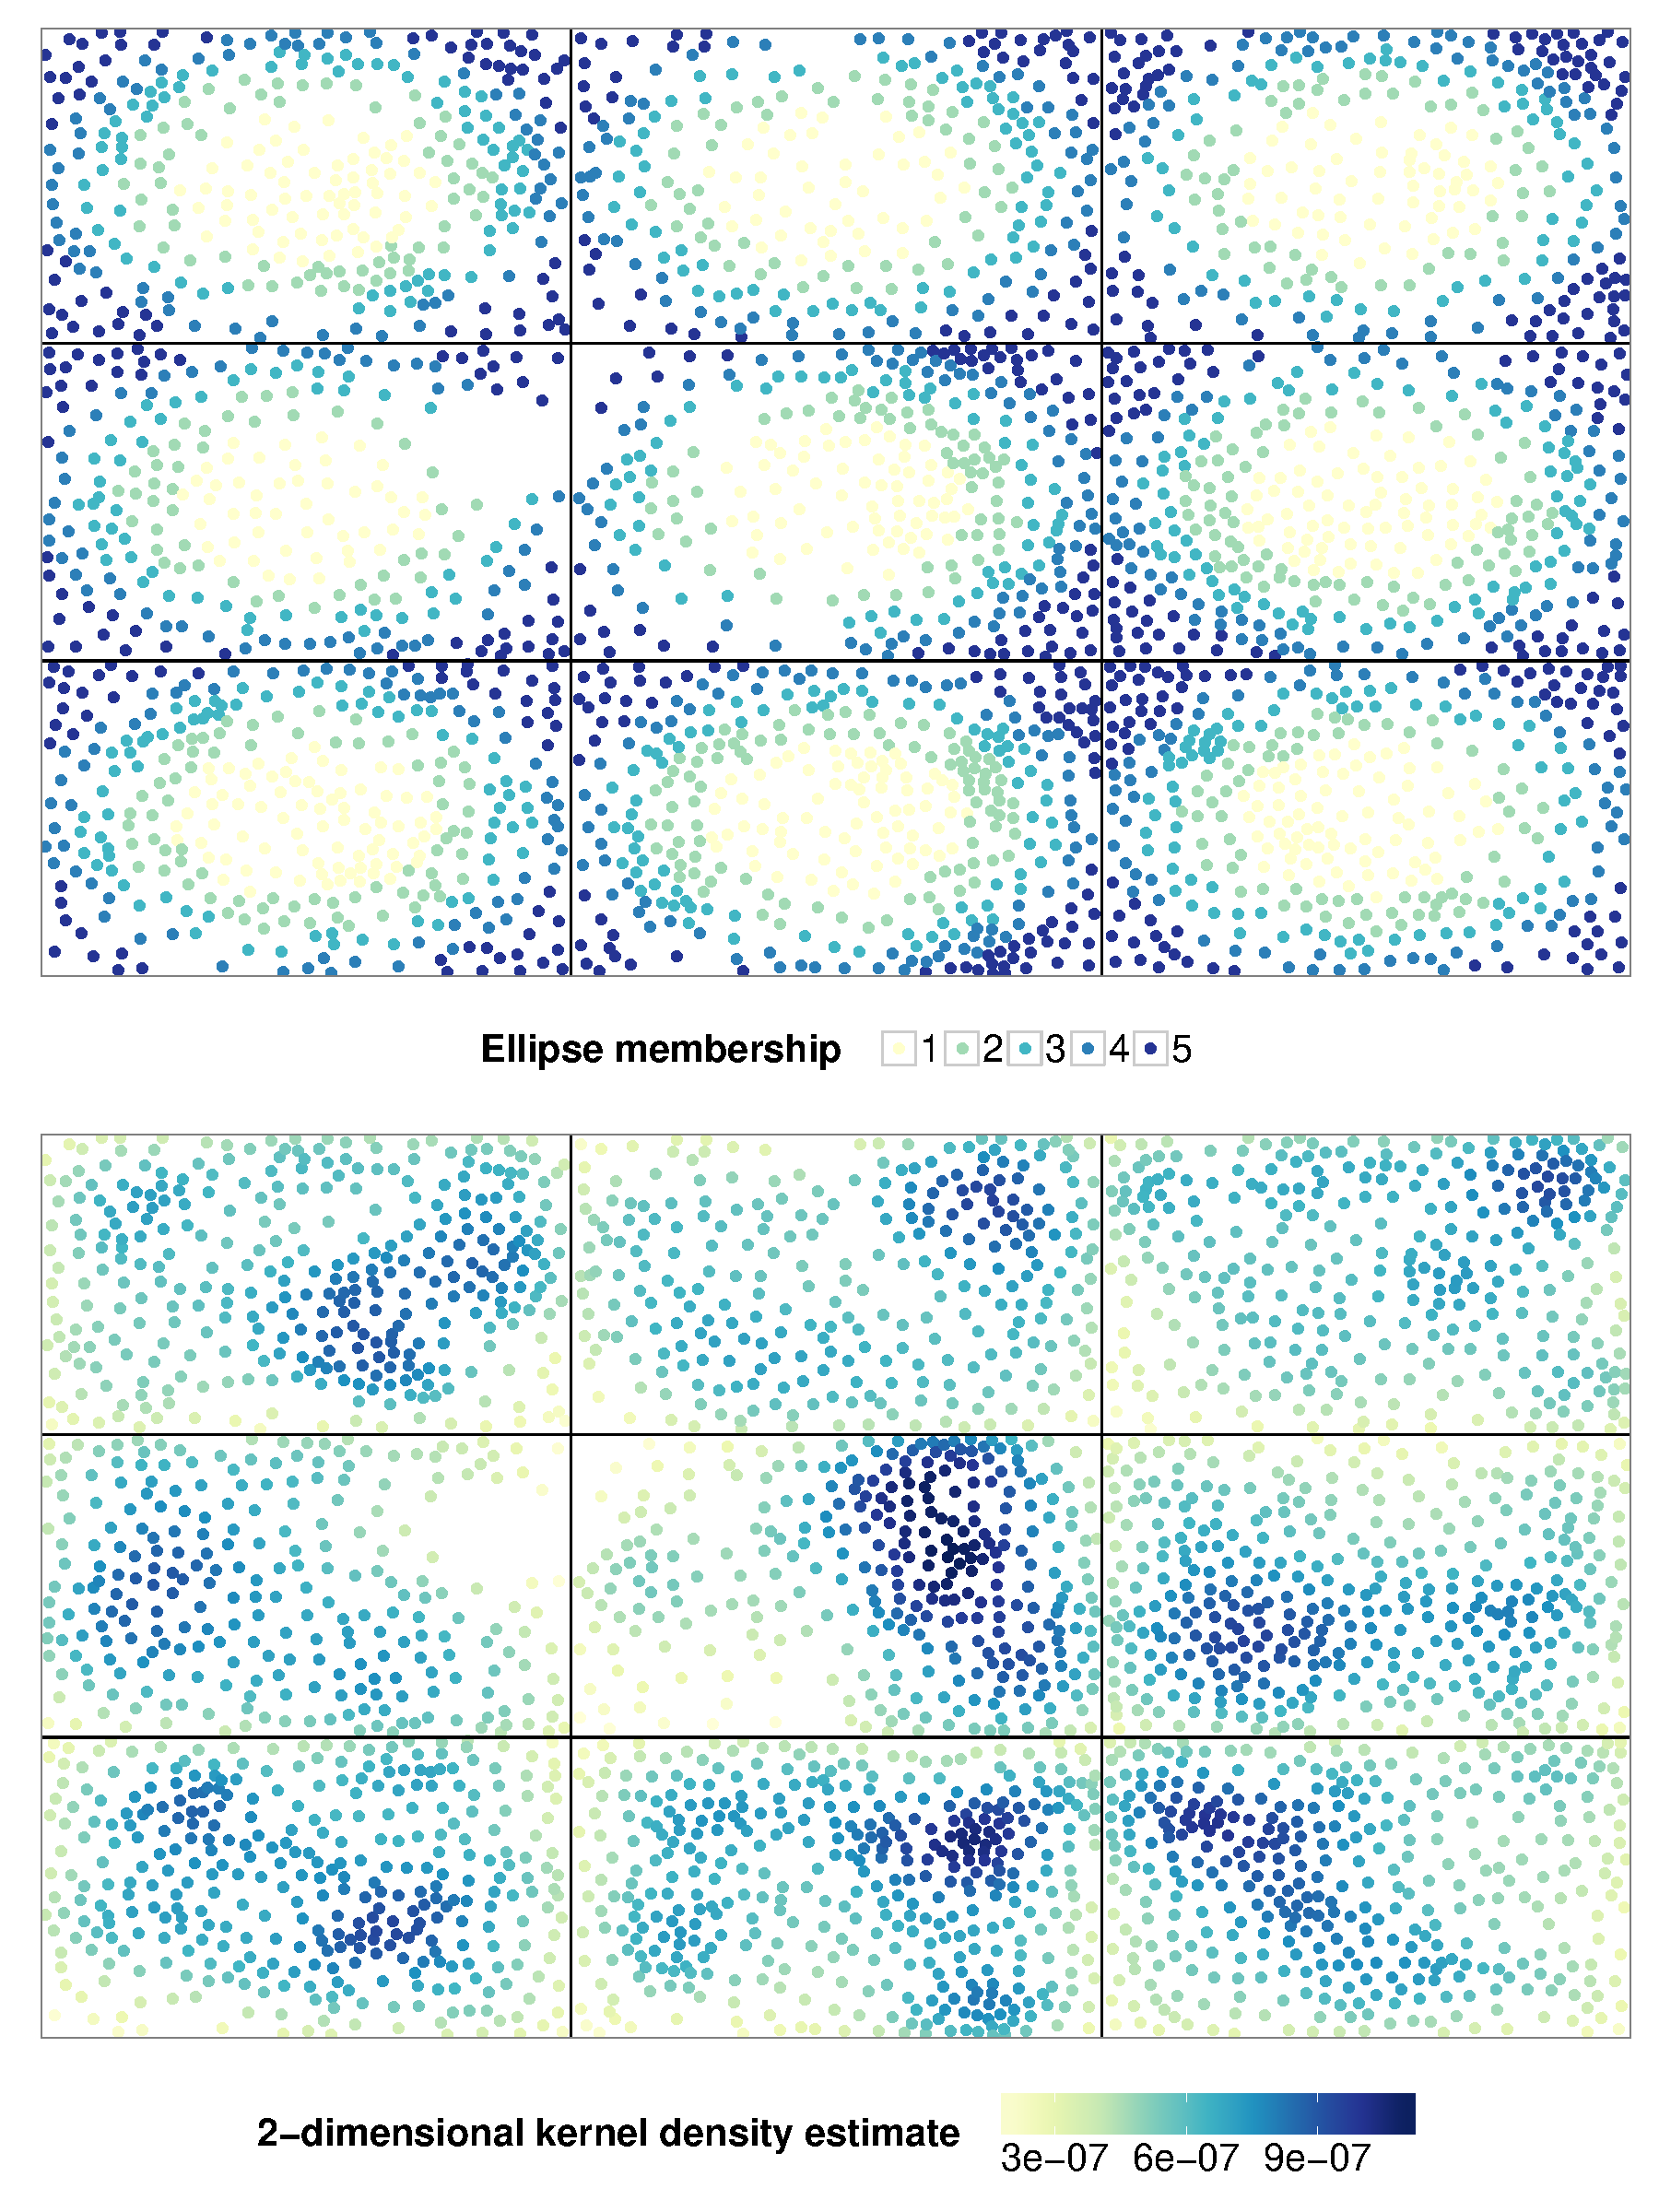
\includegraphics[width=.8\linewidth]{figures/R/augmentationFeatures-scf-augFeat_plot-1} 

}

\caption[Examples of coordinate augmentation functions as implemented in singleCellFeatures.]{Two examples of coorinate augmentation functions aiming at producing useful information from coordinates of cellular objects. The first image shows the discretized elliptic distance (5 bins of equal area) from individual image centers which could be relevant because of deteriorating optical properties of microscope lenses, while the second diagram visualized the 2-dimensional density of cellular objects, an important population context feature. Data is taken from well H6 of plate J107-2C.}\label{fig:scf-augFeat_plot}
\end{figure}


\end{knitrout}


\subsection{Feature Augmentation and Normalization}
\label{sec:scf-aug-norm}
Location features by themselves are useless, as they are represented as two vectors of individual coordinate values. If these coordinates, however are somehow contextualized, they hold the key to a considerable amount of information. Two examples of coordinate augmentation functions are visualized in figure \ref{fig:scf-augFeat_plot}. The top view is created by separating data points into concentric ellipses which might be relevant for normalizing against technical issues, such as optical properties of microscope lenses that degrade towards image borders (e.g. vignetting and sharpness). The bottom diagram shows 2-dimensional kernel density estimates as calculated by the CRAN package sm \citep{Bowman2014} which represents another population context feature as proposed by \cite{Knapp2011} and \cite{Snijder2012}.

Several additional features can be generated from object locations, all handled by \mintinline{text}{augmentCordinateFeatures}, including ellipses with respect to well center (instead of individual images centers), continuous distance from both image and well centers, as well as membership to 2-dimensional rectangular bins (both at well and image levels). Binning is accompanied by annotation with properties such as number of empty neighboring bins (see introductory example to this chapter) or their location within image and well (e.g. image border, image corner, image border that coincides with well border, image edge that is internal with respect to well, etc.).

The location of image within well can be used to generate a set of shifted coordinate features in order the describe object location not with respect to site, but well (calculated by \mintinline{text}{augmentImageLocation}). All these procedure have to be implemented in a very efficient manner, as they are used to process \tilde $10^6$ cells and cannot take more than seconds per feature in oder to be used interactively. Some aspects of this have already been covered earlier and while there is much more to discuss, the interested reader is directed to the publicly hosted \href{https://github.com/nbenn/singleCellFeatures}{source code}. All procedures can be applied at plate, well, and where applicable, at image level, owing to the S3 method dispatch system and the recursive implementation of data structures outlined in figure \ref{fig:scf-platedata}.

Another set of augmentation functions is directly aimed at data normalization. First there is \mintinline{text}{augmentAggregate}, which serves to calculate aggregate values on groups of objects (for example all cells in an image, all infected cells in a well or all pathogens throughout a plate). One argument that can be supplied as \mintinline{text}{func.aggr}, identifies an arbitrary function that produces a scalar from a vector of values (e.g. \mintinline{text}{min}, \mintinline{text}{max}, \mintinline{text}{mean}, \mintinline{text}{median}, \mintinline{text}{var}, \mintinline{text}{mad}, \mintinline{text}{sum}, etc.) and thusly performs the data summarization. An additional capability of note is the ability to include the 4 neighbors (north, east, south, west) when operating at well level in order to somewhat stabilize the results.

The function \mintinline{text}{augmentBscore} is only able to operate at plate level and produces row, column and plate effect estimates for each of the features specified by applying the \mintinline{text}{medpolish} procedure of the R stats package. Technical artifacts in \gls{hts} experiments can manifest as horizontally (for example due to a clogged pipette) or vertically striped patterns (e.g. degradation of microscope illumination) and B-scoring is a proven approach for correcting such issues. As is customary in B-scoring, control wells were originally excluded from the procedure. Unfortunately the way in which the layout of many InfectX plates is designed, this causes problems when control wells are to be used for analysis, as they occupy entire rows\slash columns for which the corresponding row and column effects are unavailable. Interleaving \gls{sirna} wells with control wells would alleviate the problem but place \gls{sirna} wells at the plate border, which is undesirable as well. Currently, control wells are included in B-scoring.

In order to perform data normalization itself, the user has two procedures at his disposal: \mintinline{text}{normalizeData}, which may be applied at every hierarchy level and \mintinline{text}{augmentMars}, which is only available to \mintinline{text}{PlateData} objects. The former function can accept regular expressions to specify the set of features it is to be applied to, as well as two sets of features that may have been generated by \mintinline{text}{augmentAggregate} for scaling and centering of the data. A small example might better convey what is possible with \mintinline{text}{normalizeData}:

\begin{rflow}
# fetch a complete plate dataset
data <- PlateData(PlateLocation("J107-2C"))
# discard any non-infected cells
data <- extractCells(data, infected=TRUE)
# regular expressions for selecting AreaShape, Intensity and Texture
# features of cellular objects
feat.sel <- c(".AreaShape_", ".Intensity_", ".Texture_")
feat.drp <- c("^Bacteria.", "^BlobBacteria.")
# calculate plate level median values for all selected features
data <- augmentAggregate(data, features=feat.sel, drop=feat.drp,
                         func.aggr="median", level="plate")
# calculate well level mad values for all selected features
data <- augmentAggregate(data, features=feat.sel, drop=feat.drp,
                         func.aggr="mad", level="well", neighbors=TRUE)
# normalize all selected values by robust Z-scoring
data <- normalizeData(data, select=feat.sel, drop=feat.drp,
                      values=".",
                      center="Aggreg_P_median$",
                      scale="Aggreg_N_mad$")
\end{rflow}

Any one of the center\slash scale parameters may be set to \mintinline{text}{NULL} and together with the flexibility of \mintinline{text}{augmentAggregate} a great range of possible normalization schemes can be applied. In this example a robust variant of Z-scoring is used, but only centering or scaling data is readily possible, as is using other summary functions (for example, \mintinline{text}{mean} and \mintinline{text}{var}, which would lead to regular Z-scoring).

One noteworthy implementation aspect is concerned with the great number of regular expressions that have to be executed. For each image, the set of selected features is iterated and within each iteration, the corresponding center and scale feature has to be found among the union of all available features (which, due to the non-destructive operation of all augmentation functions can grow up to 2000--3000). Furthermore, features are organized in a nested list (remember: at top level, they are sorted into \mintinline{text}{data.vec}, \mintinline{text}{data.mat} and \mintinline{text}{data.lst} categories and within each further subdivision into groups according to number of objects is possible). Constant traversal and matching of the same feature pairs (or triplets) is inefficient, as it is identical for all images. Therefore, a stencil of feature indices that specify locations within the nested structure, is precomputed and applied for each individual image. This optimization makes execution of a normalization scheme over a complete plate possible within \SI{90}{\second} for a setup as in the above example (only infected cells) or \SI{2}{\minute} for a full dataset.

The second normalization procedure, \mintinline{text}{augmentMars}, fits a fixed \gls{mars} model for each selected feature and returns the residuals as normalized feature values. Model fitting is performed by the CRAN package earth \citep{Hastie2015} and due to the large number of individual models that are involved, this is the most expensive operation in any singleCellFeatures analysis routine, taking on the order of \SI{25}{\minute} per plate. Normalization will be discussed more in depth in chapter \ref{sec:data-normalization}.

All augmentation and normalization functions operate in a non-destructive manner in the sense that they leave the original values intact and save results to copies of the features they were specified to operate on. In the above example, all features processed by the first application of \mintinline{text}{augmentAggregate} are saved with the added suffix \mintinline{text}{Aggreg_P_median}, which is used by \mintinline{text}{normalizeData} for identification as centering value. It is left to the user to discard sets of features that are no longer needed. While some space savings are possible, owing to the nested hierarchical model of \mintinline{text}{PlateData} structures (for example row and column effects of B-scoring do not have to be duplicated for every object, as would be the case in an entirely matrix based setup), objects holding several thousand features can become unwieldy. This is usually not a problem, as only a subset of original and derived features are needed leading to elimination of intermediate values by the user.

\subsection{Data Filtering}
Several functions for filtering datasets are available. Extraction of individual cells is possible via \mintinline{text}{extractCells} which may be applied at every plate, well or image level. Currently, the only available criterion is infection, but addition of a further group of parameters such as a vector of features, a set of order relations and corresponding thresholds could be added easily and would allow for arbitrary filtering with cellular granularity. At the next hierarchical tier, \mintinline{text}{extractImages}, available to \mintinline{text}{PlateData} and \mintinline{text}{WellData} objects, can be used to select individual images either keeping the superordinate data structure intact or discarding it, yielding a naked list. Finally, data extraction at well level is possible using \mintinline{text}{extractWells}, which owing to circumstance is only available to plate objects. Again the the user may keep the encompassing plate structure or throw it out.

Dropping or extracting a subset of features may be accomplished by calling the function \mintinline{text}{extractFeatures} on any type of \mintinline{text}{Data} structure. Either a vector of regular expressions can be used to select features, followed by application of a further vector of regular expressions for removing erroneously selected instances, or a vector of feature names can be supplied that is matched exactly. Again, for performance reasons, when run at plate scale, the large number of repeated regular expressions causes speed issues and in such cases, the feature names are worked out once for the first and reused in all subsequent wells.

The function \mintinline{text}{cleanData}, which may act on plates and wells, is currently used for eliminating image sites with very few or too many cellular objects. This measure serves to combat segmentation issues and eliminate some technical artifacts such as bad focus. Images are selected according to image-level cell count quantiles and the user can choose whether to do away with only the upper or lower 5\%, or discard data symmetrically. Having well quality annotation metadata available, the procedure is planned to be extended to also remove wells that carry the label \mintinline{text}{BAD} but as of yet this has not been a priority due to the predominance of missing labels.

Further, related functionality is provided by \mintinline{text}{makeFeatureCompatible}, which can be used to ensure that multiple \mintinline{text}{Data} objects, supplied as a list, share the same features. For dealing with data heterogeneity, the intersection of individual feature sets is computed using the base function \mintinline{text}{Reduce} and subsequently extracted from each object. In order to illustrate the brevity with which such procedures can be implemented owing to R's broad range of library functions, coupled with convenience functions available to singleCellFeatures, the source to this function is reproduced in listing \ref{lst:feature-compat}. This procedure can be applied to any combination of \mintinline{text}{PlateData}, \mintinline{text}{WellData} and \mintinline{text}{ImageData}, owing to generic functions and the S3 method dispatch system.

\subsection{Ensuring Dataset Consistency}
Despite efforts to design data structure modifying functions in such a way that prevents introducing inconsistencies, there if no formal safe-guarding and due to how S3 objects are designed, the user can do whatever he pleases (for example removing features only in a subset of wells). Therefore, several procedures exist, that can be used to ensure that some assumptions made throughout the code base (such as an identical set of features throughout a plate) still hold. Checking whether the set of features per se is complete can be done with \mintinline{text}{checkCompletenessFeature}, which has been introduced earlier as the function that checks \mintinline{text}{PlateData} objects before well caches are written and reports on the state of \mintinline{text}{MatData} caches following their retrieval.

\begin{rlisting}{float=t}{The function \mintinline{text}{makeFeatureCompatible} can be used to ensure an identical feature set among the supplied objects.}{Used for reducing the supplied list of objects to the common set of features, this function serves as an illustration of the conciseness that is possible due to R's range of library functions coupled with functionality implemented in singleCellFeatures.}{feature-compat}
\begin{rcode}
makeFeatureCompatible <- function(lst) {
  # input validation
  stopifnot(sapply(lst, function(x) any(class(x) == "Data")))
  # check objects for internal consistency
  stopifnot(sapply(lst, checkConsistency))
  # get individual feature lists
  features <- lapply(lst, getFeatureNames)
  # produce intersection of feature lists
  intersection <- Reduce(intersect, features)
  # extract intersection from each object
  res <- lapply(lst, extractFeatures, features=intersection)
  return(res)
}
\end{rcode}
\end{rlisting}

Both functions \mintinline{text}{checkCompletenessImage} and \mintinline{text}{checkCompletenessWell} are concerned with structural integrity of the respective structures in the sense that they contain the expected number of sub-structures. In case of images, two possibilities exist, which have to be handled, whereas plates are currently fixed to a 384 well-layout. Finally, \mintinline{text}{checkConsistency} is slightly more involved, as no fixed template exists that can be matched. At well level, the method builds an image-level prototype consisting of metadata such as well name, plate barcode and the structuring of features alongside feature names themselves and compares this among all images. At plate level, the procedure is applied recursively, and requires 384 additional comparisons to check coherence among wells.

Listing \ref{lst:feature-compat} contains an example application of a consistency check, which is required due to reliance on \mintinline{text}{getFeatureNames}. As this function is employed in several speed-critical settings, it simply extracts the feature set of a single image and does not check if every other image contains the same set of features. Due to the intent behind \mintinline{text}{makeFeatureCompatible} this however has to be enforced.

\subsection{Data Melting\footnote{Naming of this functionality is inspired by the pair of functions \mintinline{text}{cast} and \mintinline{text}{melt}, provided by the CRAN package reshape2 \citep{Wickham2007}.}}
One of the most important functions for every analysis procedure that relies on external tools, is \mintinline{text}{meltData} which turns the supplied \mintinline{text}{Data} structure into the smallest possible set of \mintinline{text}{data.frames} (see listing \ref{lst:meltdata}). At image level, the data representation does not have to be significantly altered apart from merging of some metadata fields into the data nodes in preparation of loss of structure conveying this information (examples include image and well indices, as well as plate barcode). At well level, the corresponding data structures are combined using \mintinline{text}{rbind} (for \mintinline{text}{vec} and \mintinline{text}{mat} features), while the \mintinline{text}{bdiag} function (from the Matrix package) is used for creating block diagonal adjacency matrices.

Well metadata is written into a special group under the \mintinline{text}{vec} node, thereby avoiding replication and consequent storage blowup (see listing \ref{lst:meltdata}, line 8 and following). A similar procedure for both storing metadata and concatenating subordinate data-structures is applied at plate level, yielding a nested list grouped by top level slots \mintinline{text}{vec}, \mintinline{text}{mat} and \mintinline{text}{lst}, which are further subdivided into \mintinline{text}{data.frames} corresponding to objects with different counts (Bacteria, BlobBacteria and Cells in case of the \mintinline{text}{mat} node shown in listing \ref{lst:meltdata}).

\afterpage{\clearpage\begin{rlisting}{nofloat}{Output structure of a complete plate as returned by \mintinline{text}{meltData}.}{While not a proper code listing, this represents a heavily truncated output view as produced by applying \mintinline{text}{str} on the result returned by \mintinline{text}{meltData} after having processed a complete plate.}{meltdata}
\begin{rcode}
List of 3
 $ vec:List of 3
  ..$ Image:'data.frame': 3456 obs. of  32 variables:
  .. ..$ Image.Count_Bacteria    : num [1:3456] 289 156 137 19 0 62 36 37 ...
  .. ..$ Image.Count_BlobBacteria: num [1:3456] 288 125 137 19 0 46 29 25 ...
  .. ..$ Well.Index              : num [1:3456] 1 1 1 1 1 1 1 1 1 2 ...
  .. .. [list output truncated]
  ..$ Well :'data.frame': 384 obs. of  15 variables:
  .. ..$ Well.Index     : num [1:384] 1 2 3 4 5 6 7 8 9 10 ...
  .. ..$ Well.Gene_ID   : chr [1:384] "523" "none" "none" "none" ...
  .. ..$ Well.siRNA_Name: chr [1:384] "ATP6V1A" "SCRAMBLED" "MOCK" "MOCK" ...
  .. .. [list output truncated]
  ..$ Plate:'data.frame': 1 obs. of  6 variables:
  .. ..$ Plate.Barcode  : chr "J101-2C"
  .. ..$ Plate.Quality  : chr "UNKNOWN"
  .. ..$ Experiment.Name: chr "BRUCELLA-DU-K1"
  .. .. [list output truncated]
 $ mat:List of 3
  ..$ Bacteria    :'data.frame':  388625 obs. of  51 variables:
  .. ..$ Bacteria.AreaShape_PerObjArea_CorrPathogen      : num [1:388625] ...
  .. ..$ Bacteria.Intensity_MassDisplacement_CorrPathogen: num [1:388625] ...
  .. ..$ Well.Index                                      : num [1:388625] ...
  .. .. [list output truncated]
  ..$ BlobBacteria:'data.frame':  222981 obs. of  7 variables:
  .. ..$ BlobBacteria.Location_Center_X: num [1:222981] 1.25 42.45 3 5 6.33 ...
  .. ..$ BlobBacteria.Location_Center_Y: num [1:222981] 130 210 119 111 138 ...
  .. ..$ Well.Index                    : num [1:222981] 1 1 1 1 1 1 1 1 1 1 ...
  .. .. [list output truncated]
  ..$ Cells       :'data.frame':  945851 obs. of  529 variables:
  .. ..$ Cells.AreaShape_Area        : num [1:945851] 141389 2104 2466 ...
  .. ..$ Cells.AreaShape_Eccentricity: num [1:945851] 0.893 0.554 0.928 ...
  .. ..$ Cells.AreaShape_EulerNumber : num [1:945851] 1 1 1 1 1 1 1 1 1 1 ...
  .. .. [list output truncated]
 $ lst:List of 2
  ..$ IdentityOfNeighbors     :List of 3
  .. ..$ Neighbors.IdentityOfNeighbors_Cells_2
                 :Formal class 'lgCMatrix' [package "Matrix"] with 6 slots
  .. .. .. ..@ i       : int [1:4746004] 8 4 7 2 6 9 19 4 9 10 ...
  .. .. .. ..@ p       : int [1:945843] 0 1 1 2 3 6 7 11 12 13 ...
  .. .. .. ..@ Dim     : int [1:2] 945842 945842
  .. .. .. ..@ Dimnames:List of 2
  .. .. .. .. ..$ : chr [1:945842] "A1_2" "A1_2" "A1_2" "A1_2" ...
  .. .. .. .. ..$ : NULL
  .. .. .. ..@ x       : logi [1:4746004] TRUE TRUE TRUE TRUE TRUE TRUE ...
  .. .. .. ..@ factors : list()
  .. .. [list output truncated]
  .. [list output truncated]
\end{rcode}

\end{rlisting}}

Acting on the structure resulting from running \mintinline{text}{meltData}, is the utility function \mintinline{text}{moveFeatures}, which is capable of relocating features between nodes \mintinline{text}{vec}, \mintinline{text}{mat} and \mintinline{text}{lst}. It can be used, for example, when a metadata feature, such as gene name needs to be available per cell, or the opposite way round, when a cellular feature should be included in the matrix representing per well features. Whether the selected data vectors have to be expanded, or collapsed, the function automatically determines which replication pattern to use or how to aggregate data (using the specified summary function) in order to meet the target dimensions. In practice, this is of great usefulness, combining space saving attributes of the molten data structure with the ability to expand user selected features for simplified interface with external procedures.

\section{Utility and Convenience Functions}
A multitude of specialized convenience functions for working with the described S3 objects were developed alongside to the functionality discussed above. Much of this code is used internally throughout the project, and where sensible, the methods are exported to the package namespace and hence made available to the user. Examples are functions for visualizing data, utilities for managing the package and cache objects, various getter functions to directly access and extract certain information from custom classes and conversion procedures for certain object pairs. Due to diversity and extent these additional features unfortunately cannot be covered in their entirety and only a selection is highlighted and briefly discussed.

\paragraph{Visualization.}
Heatmaps and box-plots can be used to visualize certain features in a plate wide context and bubble plots at a single image level are currently under development. An exemplary view, resulting from applying the function \mintinline{text}{plateHeatmap} to the feature Nuclei.AreaShape\_Area, aggregating data at well level by calculating the mean and using a logarithmic color scale is shown in figure \ref{fig:scf-heatmap}. Control wells are marked by black borders, while actual \gls{sirna} experiments are indicated by white rectangles. Tile coloring can be specified by supplying the function with a vector of colors that is interpolated to produce a gradient and the color scale is chosen by a function valued parameter (e.g. \mintinline{text}{identity} which is default, \mintinline{text}{log} or \mintinline{text}{sqrt}), while the data summary method is indicated analogously (e.g. \mintinline{text}{mean}, \mintinline{text}{median}, \mintinline{text}{var}, \mintinline{text}{mad}, etc.).

Plate-level box plots are a bit unwieldy for print media, are therefore not shown, but provide a useful method of spotting wells which might contain untrustworthy data. Bubble plots, thought for overlaying individual images with some feature data are partially implemented but the automatic image fetching from openBIS still requires some work. Such visualizations are primarily used for validating sensibility of feature data, by providing side-by side comparison with raw image data.

\begin{knitrout}
\definecolor{shadecolor}{rgb}{0.969, 0.969, 0.969}\color{fgcolor}\begin{figure}

{\centering 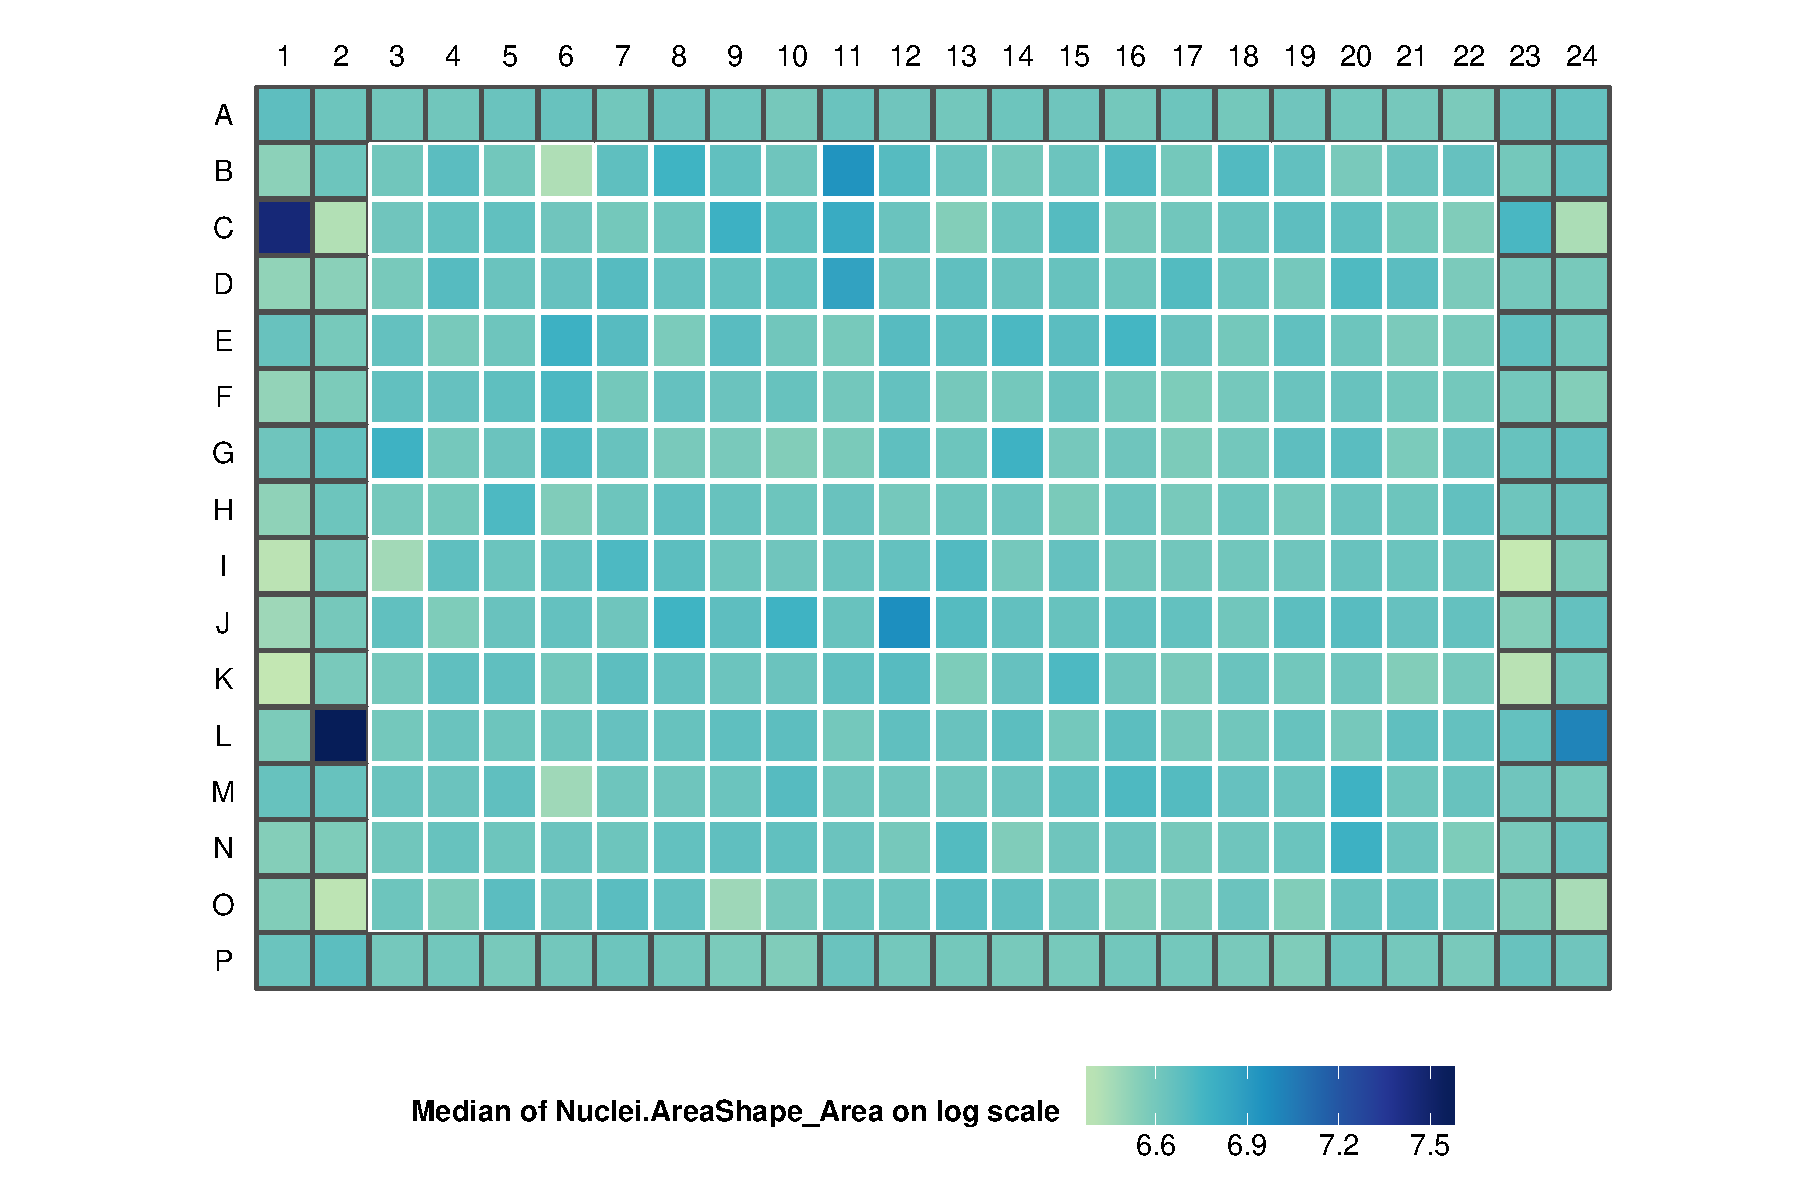
\includegraphics[width=.95\linewidth]{figures/R/heatmap-demo-scf-heatmap-1} 

}

\caption[An example heatmap plot as produced by \mintinline{text}{plateHeatmap}.]{Several visualization procedures are integrated with singelCellFeatures. In this example, the median of the feature Nuclei.AreaShape\_Area is shown on a logarithmic scale. Two parameters of \mintinline{text}{plateHeatmap} are functions so that the user can customize both, how data per well is summarized and on what scale colors are determined. The plate is J101-2C (wells C1, L2, C23 and L24 contain cell killer \gls{kif11} \gls{sirna}).}\label{fig:scf-heatmap}
\end{figure}


\end{knitrout}


\paragraph{Package utilities.}
Functions of this group have been mentioned in several places and comprise of tools for metadata coverage assessment, configuration management, cache updating and invalidation, as well as database management. A report on the discrepancy between plates that have single cell features available and datasets that are represented by metadata is generated each time the package is attached to an R session (using the \mintinline{text}{.onLoad} hook). The corresponding function, run as \mintinline{text}{wellDatabaseCoverage(TRUE)} can be used to display a detailed overview of current metadata coverage at well level which is particularly important for searching.

Configuration management relies on a yaml based file used storing system specific parameters (see section \ref{sec:install-package}). Setter functions, as well as getters for location and content, in addition to an initiation routine that sets up an empty template for user editing, are available for its manipulation and access.

In order to curate the lookup tables used for search and various speed critical, metadata dependent processes, each database type has a corresponding update function available (\mintinline{text}{updateDatabaseFeatures}, \mintinline{text}{updateDatabasePlate} and \mintinline{text}{updateDatabaseWells}). As all metadata available to singleCellFeatures is static and does not reflect new additions to openBIS, section \ref{sec:update-metadata} describes how to update the underlying files and the above tools can recreate the databases using updated source data.

While cache-related functionality has primarily been covered from a perspective of creation and retrieval, several additional functions for managing the set of cached objects are at the users disposal. Metadata and well caches can be flushed (rebuilding is comparably cheap) and reports on the extent of plate level caches can be compiled. Moreover, \mintinline{text}{rebuildAllMatDataCaches} implements a procedure that iterates all plate cache objects and determines if any improvements are available. This can be used, for example after batch-downloading many plates to trigger retry of features that failed to import in applicable plates, or in case some features did not download, selectively initiate re-fetching. A further application is if new features become available, the function can be used to specifically start the respective downloads and imports into existing objects eliminating the need of having to re-process affected plates completely (which is an expensive operation).

Furthermore, for the package to be usable in a cluster environment, resource allocation has to be respected. Parallelized sections are using foreach \citep{Weston2014} alongside the doParallel backend \citep{Weston2014a} and it needs to be ensured that forked processes only run on the allowed cores. The function \mintinline{text}{getNumCores}, for example, can be used to determine the number of available cores by either reading the corresponding environmental variable set by Platform LSF, or by using \mintinline{text}{detectCores} of doParallel.

\begin{rlisting}{float=t}{A convenience function that converts its argument into a \mintinline{text}{PlateLocation} object.}{Many convenience functions are available to singleCellFeatures, one of which can be used to convert its argument into a \mintinline{text}{PlateLocation} object. A further example of such a simple, single purpose method is the getter function \mintinline{text}{getBarcode}, which extract the barcode from the object it is called upon.}{convert}
\begin{rcode}
convertToPlateLocation <- function(x) {
  UseMethod("convertToPlateLocation", x)
}

convertToPlateLocation.DataLocation <- function(x) {
  barcode <- getBarcode(x)
  return(PlateLocation(barcode))
}

convertToPlateLocation.Data <- function(x) {
  barcode <- getBarcode(x)
  return(PlateLocation(barcode))
}

convertToPlateLocation.PlateAggregate <- function(x) {
  return(x$plate)
}

convertToPlateLocation.default <- function(x) {
  stop("can only deal with PlateData/MatData/WellLocation objects.")
}
\end{rcode}
\end{rlisting}

\paragraph{Convenience functions.}
This section covers a diverse range of methods including many getters for S3 objects and short, narrow purpose functions for common tasks. It is unfitting to describe these tools in their entirety and the interested reader is encouraged to look at the publicly hosted source code, or look though the manual pages that come with the package and are browsable through the R help system. Listing \ref{lst:convert} shows one instance of such a function which can be used to create a \mintinline{text}{PlateLocation} object out of the supplied data structure, thereby converting the argument into a plate location specification. The example on page \pageref{ex:dataobject-instantiation} provides a real-world application of such a conversion function.

The reasoning for using multiple description attributes for objects can be illustrated by means of this code excerpt:\footnote{As a reminder, for instance, both \mintinline{text}{PlateLocation} and \mintinline{text}{WellLocation} are also \mintinline{text}{DataLocation} objects and the same pattern holds for other groups of S3 classes.} As the function \mintinline{text}{getBarcode} (one of the aforementioned getter functions) is defined for all \mintinline{text}{Data} classes, four functions acting on \mintinline{text}{MatData}, \mintinline{text}{PlateData}, \mintinline{text}{WellData} and \mintinline{text}{ImageData} can be written as one by creating this additional level of hierarchy in object type naming, thereby reducing redundant code. In this case, one could even combine the functions that act on \mintinline{text}{DataLocation} and \mintinline{text}{Data} objects if an attribute grouping those classes were available. However, to avoid overly complex attribute relationships, only functionally related classes are gathered.

\paragraph{Interface to \acrshort{glm} routines.}
Currently still under development, several functions that interface with \gls{glm} routines are available to the user. Originally intended for building a model that discriminates two gene knockdown experiments based on single cell features, the function \mintinline{text}{prepareDataforGlm} can take two lists of wells and make the data ready for analysis with \gls{glm} by concatenating and annotating the wells with a response vector. Additional options are sampling based splitting of data into testing and training sets and dropping of features that by themselves separate the data into the two knockdown groups.

Due to issues in logistic regression, caused by data that is separated into the two groups that are modeled by a hyperplane, \mintinline{text}{analyzeSeparation} can be used for preliminary investigation of this aspect. The procedure will first check if individual features separate the data, followed by looking at all $n \choose 2$ pairs of features. Unordered \textit{k}-tuples may be explored up to a user defined threshold but with several 100 features to be considered, the number of sets resulting from $k > 2$ becomes prohibitively large and the function will skip iteration k and above if ${n \choose k} > 250000$. In a final step, all features are considered simultaneously, solving the problem with a linear programming approach, using the CRAN package lpSolveAPI \citep{Konis2007,Konis2014}. A further data issue that has to be dealt with is rank deficiency and the procedure \mintinline{text}{makeRankFull} can be used in this capacity. Features that either have zero variance or comprise of highly correlated columns, are removed prior to analysis.

A parallelized function for investigating the stability of the largest n coefficients in \gls{glm}, the set of features as determined by stepwise \gls{glm}, or the set of nonzero coefficients in regularized \gls{glm} analysis is available as the function \mintinline{text}{glmBootstrapStability}. For both stepwise and plain \gls{glm}, the functions \mintinline{text}{glm} and \mintinline{text}{step} of the R stats package are used, while regularized fitting is performed by \mintinline{text}{glmnet} \citep{Friedman2010a}. A user specified fraction of the data (default 0.7) is sampled in each iteration and the resulting coefficients are stored for subsequent counting and tabulation. Unfortunately, there currently are unresolved issues regarding data normalization, making this type of analysis infeasible. Therefore all \gls{glm} oriented routines are subject to change.

